% Release Gates for LLM Applications
% Build: make final   (real results)   |   make draft   (synthetic fixture, watermarked)
% AUTHOR: confirm full name and affiliation before submission.
\documentclass[10pt,a4paper]{article}

\usepackage[margin=1in]{geometry}
\usepackage[T1]{fontenc}
\usepackage[utf8]{inputenc}
\usepackage{lmodern}
\usepackage{microtype}
\usepackage{amsmath,amssymb}
\usepackage{booktabs}
\usepackage{graphicx}
\usepackage{adjustbox}
\usepackage{xcolor}
\usepackage{tikz}
\usetikzlibrary{arrows.meta,positioning,calc}
\usepackage[ruled,linesnumbered,noend]{algorithm2e}
\usepackage{caption}
\usepackage{subcaption}
\usepackage{enumitem}
\usepackage{url}
\usepackage[backend=biber,style=numeric,sorting=none,maxbibnames=9,giveninits=true]{biblatex}
\addbibresource{refs.bib}
\usepackage[colorlinks=true,linkcolor=blue!50!black,citecolor=blue!50!black,urlcolor=blue!50!black]{hyperref}
\usepackage[capitalise,noabbrev]{cleveref}

\newcommand{\resultsmode}{final}
\newcommand{\resultsdate}{2026-11-05}
\newcommand{\resultspath}{packages/evals/results/2026-11-05/metrics.json}
\newcommand{\oodsources}{jackhhao/jailbreak-classification, lakera/gandalf\_ignore\_instructions}
\newcommand{\nraw}{80277}
\newcommand{\ndedupe}{78908}
\newcommand{\ncaps}{10101}
\newcommand{\ntrain}{6689}
\newcommand{\ntrainattack}{2610}
\newcommand{\ntrainbenign}{4079}
\newcommand{\nval}{836}
\newcommand{\ntest}{836}
\newcommand{\ntestood}{1740}
\newcommand{\ntestoodattack}{1110}
\newcommand{\ntestoodbenign}{630}
\newcommand{\ntestevident}{278}
\newcommand{\ntestperturbed}{4340}
\newcommand{\ntestperturbedattack}{3200}
\newcommand{\nperturbtype}{400}
\newcommand{\bestooddetector}{ProtectAI DeBERTa v2}
\newcommand{\bestoodauroc}{0.998}
\newcommand{\deferralvariant}{analytic cost model with the measured regex (0.09 ms) and classifier latencies}
\newcommand{\mregexlowtestauroc}{0.644}
\newcommand{\mregexlowtestrecall}{0.291}
\newcommand{\mregexlowtestprecision}{0.990}
\newcommand{\mregexlowtestfone}{0.450}
\newcommand{\mregexlowtestfpr}{0.002}
\newcommand{\mregexlowtestap}{0.561}
\newcommand{\mregexlowtestfpratrecall}{1.000}
\newcommand{\mregexlowtestlatency}{0.08}
\newcommand{\mregexlowtestlatencypninefive}{0.20}
\newcommand{\mregexlowtestlmauroc}{0.649}
\newcommand{\mregexlowtestlmfone}{0.463}
\newcommand{\mregexlowtestoodauroc}{0.790}
\newcommand{\mregexlowtestoodrecall}{0.584}
\newcommand{\mregexlowtestoodprecision}{0.991}
\newcommand{\mregexlowtestoodfone}{0.735}
\newcommand{\mregexlowtestoodfpr}{0.010}
\newcommand{\mregexlowtestoodap}{0.849}
\newcommand{\mregexlowtestoodfpratrecall}{1.000}
\newcommand{\mregexlowtestoodlatency}{0.08}
\newcommand{\mregexlowtestoodlatencypninefive}{0.29}
\newcommand{\mregexlowtestoodlmauroc}{0.860}
\newcommand{\mregexlowtestoodlmfone}{0.836}
\newcommand{\mregexlowtestevidentauroc}{0.935}
\newcommand{\mregexlowtestevidentrecall}{0.871}
\newcommand{\mregexlowtestevidentprecision}{1.000}
\newcommand{\mregexlowtestevidentfone}{0.931}
\newcommand{\mregexlowtestevidentfpr}{0.000}
\newcommand{\mregexlowtestevidentap}{0.939}
\newcommand{\mregexlowtestevidentfpratrecall}{1.000}
\newcommand{\mregexlowtestevidentlatency}{0.02}
\newcommand{\mregexlowtestevidentlatencypninefive}{0.03}
\newcommand{\mregexlowtestevidentlmauroc}{0.944}
\newcommand{\mregexlowtestevidentlmfone}{0.941}
\newcommand{\mregexlowtestperturbedauroc}{0.591}
\newcommand{\mregexlowtestperturbedrecall}{0.188}
\newcommand{\mregexlowtestperturbedprecision}{0.989}
\newcommand{\mregexlowtestperturbedfone}{0.316}
\newcommand{\mregexlowtestperturbedfpr}{0.006}
\newcommand{\mregexlowtestperturbedap}{0.785}
\newcommand{\mregexlowtestperturbedfpratrecall}{1.000}
\newcommand{\mregexlowtestperturbedlatency}{0.06}
\newcommand{\mregexlowtestperturbedlatencypninefive}{0.27}
\newcommand{\mregexlowtestperturbedlmauroc}{0.618}
\newcommand{\mregexlowtestperturbedlmfone}{0.388}
\newcommand{\mregexlowtestoodfprpct}{1.0}
\newcommand{\mpregexlowtokenbreakspace}{0.107}
\newcommand{\mpregexlowtokenbreakhyphen}{0.110}
\newcommand{\mpregexlowzerowidth}{0.087}
\newcommand{\mpregexlowhomoglyph}{0.087}
\newcommand{\mpregexlowleetspeak}{0.090}
\newcommand{\mpregexlowcaseflip}{0.510}
\newcommand{\mpregexlowbenignprefix}{0.512}
\newcommand{\mpregexlowbasesixfourwrap}{0.000}
\newcommand{\mregexmediumtestauroc}{0.649}
\newcommand{\mregexmediumtestrecall}{0.301}
\newcommand{\mregexmediumtestprecision}{0.990}
\newcommand{\mregexmediumtestfone}{0.461}
\newcommand{\mregexmediumtestfpr}{0.002}
\newcommand{\mregexmediumtestap}{0.566}
\newcommand{\mregexmediumtestfpratrecall}{1.000}
\newcommand{\mregexmediumtestlatency}{0.10}
\newcommand{\mregexmediumtestlatencypninefive}{0.21}
\newcommand{\mregexmediumtestlmauroc}{0.654}
\newcommand{\mregexmediumtestlmfone}{0.475}
\newcommand{\mregexmediumtestoodauroc}{0.799}
\newcommand{\mregexmediumtestoodrecall}{0.604}
\newcommand{\mregexmediumtestoodprecision}{0.990}
\newcommand{\mregexmediumtestoodfone}{0.750}
\newcommand{\mregexmediumtestoodfpr}{0.011}
\newcommand{\mregexmediumtestoodap}{0.856}
\newcommand{\mregexmediumtestoodfpratrecall}{1.000}
\newcommand{\mregexmediumtestoodlatency}{0.09}
\newcommand{\mregexmediumtestoodlatencypninefive}{0.31}
\newcommand{\mregexmediumtestoodlmauroc}{0.865}
\newcommand{\mregexmediumtestoodlmfone}{0.844}
\newcommand{\mregexmediumtestevidentauroc}{0.992}
\newcommand{\mregexmediumtestevidentrecall}{0.986}
\newcommand{\mregexmediumtestevidentprecision}{0.973}
\newcommand{\mregexmediumtestevidentfone}{0.980}
\newcommand{\mregexmediumtestevidentfpr}{0.031}
\newcommand{\mregexmediumtestevidentap}{0.991}
\newcommand{\mregexmediumtestevidentfpratrecall}{0.031}
\newcommand{\mregexmediumtestevidentlatency}{0.02}
\newcommand{\mregexmediumtestevidentlatencypninefive}{0.03}
\newcommand{\mregexmediumtestevidentlmauroc}{0.995}
\newcommand{\mregexmediumtestevidentlmfone}{0.980}
\newcommand{\mregexmediumtestperturbedauroc}{0.597}
\newcommand{\mregexmediumtestperturbedrecall}{0.200}
\newcommand{\mregexmediumtestperturbedprecision}{0.988}
\newcommand{\mregexmediumtestperturbedfone}{0.332}
\newcommand{\mregexmediumtestperturbedfpr}{0.007}
\newcommand{\mregexmediumtestperturbedap}{0.788}
\newcommand{\mregexmediumtestperturbedfpratrecall}{1.000}
\newcommand{\mregexmediumtestperturbedlatency}{0.08}
\newcommand{\mregexmediumtestperturbedlatencypninefive}{0.35}
\newcommand{\mregexmediumtestperturbedlmauroc}{0.621}
\newcommand{\mregexmediumtestperturbedlmfone}{0.396}
\newcommand{\mregexmediumtestoodfprpct}{1.1}
\newcommand{\mpregexmediumtokenbreakspace}{0.120}
\newcommand{\mpregexmediumtokenbreakhyphen}{0.120}
\newcommand{\mpregexmediumzerowidth}{0.098}
\newcommand{\mpregexmediumhomoglyph}{0.095}
\newcommand{\mpregexmediumleetspeak}{0.098}
\newcommand{\mpregexmediumcaseflip}{0.532}
\newcommand{\mpregexmediumbenignprefix}{0.535}
\newcommand{\mpregexmediumbasesixfourwrap}{0.000}
\newcommand{\mregexhightestauroc}{0.654}
\newcommand{\mregexhightestrecall}{0.310}
\newcommand{\mregexhightestprecision}{0.990}
\newcommand{\mregexhightestfone}{0.472}
\newcommand{\mregexhightestfpr}{0.002}
\newcommand{\mregexhightestap}{0.572}
\newcommand{\mregexhightestfpratrecall}{1.000}
\newcommand{\mregexhightestlatency}{0.11}
\newcommand{\mregexhightestlatencypninefive}{0.24}
\newcommand{\mregexhightestlmauroc}{0.658}
\newcommand{\mregexhightestlmfone}{0.484}
\newcommand{\mregexhightestoodauroc}{0.801}
\newcommand{\mregexhightestoodrecall}{0.608}
\newcommand{\mregexhightestoodprecision}{0.990}
\newcommand{\mregexhightestoodfone}{0.753}
\newcommand{\mregexhightestoodfpr}{0.011}
\newcommand{\mregexhightestoodap}{0.857}
\newcommand{\mregexhightestoodfpratrecall}{1.000}
\newcommand{\mregexhightestoodlatency}{0.11}
\newcommand{\mregexhightestoodlatencypninefive}{0.41}
\newcommand{\mregexhightestoodlmauroc}{0.869}
\newcommand{\mregexhightestoodlmfone}{0.848}
\newcommand{\mregexhightestevidentauroc}{0.998}
\newcommand{\mregexhightestevidentrecall}{1.000}
\newcommand{\mregexhightestevidentprecision}{0.919}
\newcommand{\mregexhightestevidentfone}{0.958}
\newcommand{\mregexhightestevidentfpr}{0.099}
\newcommand{\mregexhightestevidentap}{0.997}
\newcommand{\mregexhightestevidentfpratrecall}{0.031}
\newcommand{\mregexhightestevidentlatency}{0.03}
\newcommand{\mregexhightestevidentlatencypninefive}{0.06}
\newcommand{\mregexhightestevidentlmauroc}{0.998}
\newcommand{\mregexhightestevidentlmfone}{0.951}
\newcommand{\mregexhightestperturbedauroc}{0.689}
\newcommand{\mregexhightestperturbedrecall}{0.385}
\newcommand{\mregexhightestperturbedprecision}{0.994}
\newcommand{\mregexhightestperturbedfone}{0.555}
\newcommand{\mregexhightestperturbedfpr}{0.007}
\newcommand{\mregexhightestperturbedap}{0.836}
\newcommand{\mregexhightestperturbedfpratrecall}{1.000}
\newcommand{\mregexhightestperturbedlatency}{0.10}
\newcommand{\mregexhightestperturbedlatencypninefive}{0.45}
\newcommand{\mregexhightestperturbedlmauroc}{0.723}
\newcommand{\mregexhightestperturbedlmfone}{0.621}
\newcommand{\mregexhightestoodfprpct}{1.1}
\newcommand{\mpregexhightokenbreakspace}{0.128}
\newcommand{\mpregexhightokenbreakhyphen}{0.128}
\newcommand{\mpregexhighzerowidth}{0.105}
\newcommand{\mpregexhighhomoglyph}{0.868}
\newcommand{\mpregexhighleetspeak}{0.105}
\newcommand{\mpregexhighcaseflip}{0.542}
\newcommand{\mpregexhighbenignprefix}{0.542}
\newcommand{\mpregexhighbasesixfourwrap}{0.665}
\newcommand{\mlengthonlytestauroc}{0.745}
\newcommand{\mlengthonlytestrecall}{0.724}
\newcommand{\mlengthonlytestprecision}{0.576}
\newcommand{\mlengthonlytestfone}{0.641}
\newcommand{\mlengthonlytestfpr}{0.341}
\newcommand{\mlengthonlytestap}{0.596}
\newcommand{\mlengthonlytestfpratrecall}{0.633}
\newcommand{\mlengthonlytestlatency}{0.00}
\newcommand{\mlengthonlytestlatencypninefive}{0.00}
\newcommand{\mlengthonlytestlmauroc}{0.676}
\newcommand{\mlengthonlytestlmfone}{0.668}
\newcommand{\mlengthonlytestoodauroc}{0.336}
\newcommand{\mlengthonlytestoodrecall}{0.508}
\newcommand{\mlengthonlytestoodprecision}{0.553}
\newcommand{\mlengthonlytestoodfone}{0.530}
\newcommand{\mlengthonlytestoodfpr}{0.722}
\newcommand{\mlengthonlytestoodap}{0.538}
\newcommand{\mlengthonlytestoodfpratrecall}{0.987}
\newcommand{\mlengthonlytestoodlatency}{0.00}
\newcommand{\mlengthonlytestoodlatencypninefive}{0.00}
\newcommand{\mlengthonlytestoodlmauroc}{0.577}
\newcommand{\mlengthonlytestoodlmfone}{0.623}
\newcommand{\mlengthonlytestevidentauroc}{0.728}
\newcommand{\mlengthonlytestevidentrecall}{0.265}
\newcommand{\mlengthonlytestevidentprecision}{0.848}
\newcommand{\mlengthonlytestevidentfone}{0.404}
\newcommand{\mlengthonlytestevidentfpr}{0.053}
\newcommand{\mlengthonlytestevidentap}{0.771}
\newcommand{\mlengthonlytestevidentfpratrecall}{0.878}
\newcommand{\mlengthonlytestevidentlatency}{0.00}
\newcommand{\mlengthonlytestevidentlatencypninefive}{0.00}
\newcommand{\mlengthonlytestevidentlmauroc}{0.746}
\newcommand{\mlengthonlytestevidentlmfone}{0.435}
\newcommand{\mlengthonlytestperturbedauroc}{0.561}
\newcommand{\mlengthonlytestperturbedrecall}{0.618}
\newcommand{\mlengthonlytestperturbedprecision}{0.759}
\newcommand{\mlengthonlytestperturbedfone}{0.681}
\newcommand{\mlengthonlytestperturbedfpr}{0.552}
\newcommand{\mlengthonlytestperturbedap}{0.800}
\newcommand{\mlengthonlytestperturbedfpratrecall}{0.904}
\newcommand{\mlengthonlytestperturbedlatency}{0.00}
\newcommand{\mlengthonlytestperturbedlatencypninefive}{0.00}
\newcommand{\mlengthonlytestperturbedlmauroc}{0.641}
\newcommand{\mlengthonlytestperturbedlmfone}{0.628}
\newcommand{\mlengthonlytestoodfprpct}{72.2}
\newcommand{\mplengthonlytokenbreakspace}{0.295}
\newcommand{\mplengthonlytokenbreakhyphen}{0.655}
\newcommand{\mplengthonlyzerowidth}{0.655}
\newcommand{\mplengthonlyhomoglyph}{0.552}
\newcommand{\mplengthonlyleetspeak}{0.552}
\newcommand{\mplengthonlycaseflip}{0.552}
\newcommand{\mplengthonlybenignprefix}{0.682}
\newcommand{\mplengthonlybasesixfourwrap}{1.000}
\newcommand{\mngramlrtestauroc}{0.996}
\newcommand{\mngramlrtestrecall}{0.948}
\newcommand{\mngramlrtestprecision}{0.984}
\newcommand{\mngramlrtestfone}{0.966}
\newcommand{\mngramlrtestfpr}{0.010}
\newcommand{\mngramlrtestap}{0.994}
\newcommand{\mngramlrtestfpratrecall}{0.012}
\newcommand{\mngramlrtestlatency}{0.33}
\newcommand{\mngramlrtestlatencypninefive}{0.53}
\newcommand{\mngramlrtestlmauroc}{0.995}
\newcommand{\mngramlrtestlmfone}{0.965}
\newcommand{\mngramlrtestoodauroc}{0.978}
\newcommand{\mngramlrtestoodrecall}{0.932}
\newcommand{\mngramlrtestoodprecision}{0.952}
\newcommand{\mngramlrtestoodfone}{0.942}
\newcommand{\mngramlrtestoodfpr}{0.083}
\newcommand{\mngramlrtestoodap}{0.989}
\newcommand{\mngramlrtestoodfpratrecall}{0.106}
\newcommand{\mngramlrtestoodlatency}{0.62}
\newcommand{\mngramlrtestoodlatencypninefive}{0.86}
\newcommand{\mngramlrtestoodlmauroc}{0.993}
\newcommand{\mngramlrtestoodlmfone}{0.954}
\newcommand{\mngramlrtestevidentauroc}{0.911}
\newcommand{\mngramlrtestevidentrecall}{0.755}
\newcommand{\mngramlrtestevidentprecision}{0.902}
\newcommand{\mngramlrtestevidentfone}{0.822}
\newcommand{\mngramlrtestevidentfpr}{0.092}
\newcommand{\mngramlrtestevidentap}{0.928}
\newcommand{\mngramlrtestevidentfpratrecall}{0.466}
\newcommand{\mngramlrtestevidentlatency}{0.10}
\newcommand{\mngramlrtestevidentlatencypninefive}{0.17}
\newcommand{\mngramlrtestevidentlmauroc}{0.917}
\newcommand{\mngramlrtestevidentlmfone}{0.840}
\newcommand{\mngramlrtestperturbedauroc}{0.930}
\newcommand{\mngramlrtestperturbedrecall}{0.727}
\newcommand{\mngramlrtestperturbedprecision}{0.976}
\newcommand{\mngramlrtestperturbedfone}{0.833}
\newcommand{\mngramlrtestperturbedfpr}{0.050}
\newcommand{\mngramlrtestperturbedap}{0.974}
\newcommand{\mngramlrtestperturbedfpratrecall}{0.393}
\newcommand{\mngramlrtestperturbedlatency}{0.47}
\newcommand{\mngramlrtestperturbedlatencypninefive}{0.66}
\newcommand{\mngramlrtestperturbedlmauroc}{0.927}
\newcommand{\mngramlrtestperturbedlmfone}{0.819}
\newcommand{\mngramlrtestoodfprpct}{8.3}
\newcommand{\mpngramlrtokenbreakspace}{0.873}
\newcommand{\mpngramlrtokenbreakhyphen}{0.833}
\newcommand{\mpngramlrzerowidth}{0.882}
\newcommand{\mpngramlrhomoglyph}{0.828}
\newcommand{\mpngramlrleetspeak}{0.613}
\newcommand{\mpngramlrcaseflip}{0.938}
\newcommand{\mpngramlrbenignprefix}{0.830}
\newcommand{\mpngramlrbasesixfourwrap}{0.018}
\newcommand{\mprotectaidebertavtwotestauroc}{0.986}
\newcommand{\mprotectaidebertavtwotestrecall}{0.813}
\newcommand{\mprotectaidebertavtwotestprecision}{0.996}
\newcommand{\mprotectaidebertavtwotestfone}{0.895}
\newcommand{\mprotectaidebertavtwotestfpr}{0.002}
\newcommand{\mprotectaidebertavtwotestap}{0.985}
\newcommand{\mprotectaidebertavtwotestfpratrecall}{0.027}
\newcommand{\mprotectaidebertavtwotestlatency}{294}
\newcommand{\mprotectaidebertavtwotestlatencypninefive}{664}
\newcommand{\mprotectaidebertavtwotestlmauroc}{0.984}
\newcommand{\mprotectaidebertavtwotestlmfone}{0.888}
\newcommand{\mprotectaidebertavtwotestoodauroc}{0.998}
\newcommand{\mprotectaidebertavtwotestoodrecall}{0.983}
\newcommand{\mprotectaidebertavtwotestoodprecision}{0.996}
\newcommand{\mprotectaidebertavtwotestoodfone}{0.990}
\newcommand{\mprotectaidebertavtwotestoodfpr}{0.006}
\newcommand{\mprotectaidebertavtwotestoodap}{0.998}
\newcommand{\mprotectaidebertavtwotestoodfpratrecall}{0.002}
\newcommand{\mprotectaidebertavtwotestoodlatency}{373}
\newcommand{\mprotectaidebertavtwotestoodlatencypninefive}{617}
\newcommand{\mprotectaidebertavtwotestoodlmauroc}{0.997}
\newcommand{\mprotectaidebertavtwotestoodlmfone}{0.976}
\newcommand{\mprotectaidebertavtwotestevidentauroc}{0.965}
\newcommand{\mprotectaidebertavtwotestevidentrecall}{0.871}
\newcommand{\mprotectaidebertavtwotestevidentprecision}{0.948}
\newcommand{\mprotectaidebertavtwotestevidentfone}{0.908}
\newcommand{\mprotectaidebertavtwotestevidentfpr}{0.053}
\newcommand{\mprotectaidebertavtwotestevidentap}{0.960}
\newcommand{\mprotectaidebertavtwotestevidentfpratrecall}{0.168}
\newcommand{\mprotectaidebertavtwotestevidentlatency}{15.37}
\newcommand{\mprotectaidebertavtwotestevidentlatencypninefive}{28.79}
\newcommand{\mprotectaidebertavtwotestevidentlmauroc}{0.964}
\newcommand{\mprotectaidebertavtwotestevidentlmfone}{0.901}
\newcommand{\mprotectaidebertavtwotestperturbedauroc}{0.996}
\newcommand{\mprotectaidebertavtwotestperturbedrecall}{0.932}
\newcommand{\mprotectaidebertavtwotestperturbedprecision}{0.998}
\newcommand{\mprotectaidebertavtwotestperturbedfone}{0.964}
\newcommand{\mprotectaidebertavtwotestperturbedfpr}{0.004}
\newcommand{\mprotectaidebertavtwotestperturbedap}{0.998}
\newcommand{\mprotectaidebertavtwotestperturbedfpratrecall}{0.007}
\newcommand{\mprotectaidebertavtwotestperturbedlatency}{389}
\newcommand{\mprotectaidebertavtwotestperturbedlatencypninefive}{609}
\newcommand{\mprotectaidebertavtwotestperturbedlmauroc}{0.996}
\newcommand{\mprotectaidebertavtwotestperturbedlmfone}{0.968}
\newcommand{\mprotectaidebertavtwotestoodfprpct}{0.6}
\newcommand{\mpprotectaidebertavtwotokenbreakspace}{0.917}
\newcommand{\mpprotectaidebertavtwotokenbreakhyphen}{0.932}
\newcommand{\mpprotectaidebertavtwozerowidth}{0.932}
\newcommand{\mpprotectaidebertavtwohomoglyph}{0.927}
\newcommand{\mpprotectaidebertavtwoleetspeak}{0.835}
\newcommand{\mpprotectaidebertavtwocaseflip}{0.983}
\newcommand{\mpprotectaidebertavtwobenignprefix}{0.927}
\newcommand{\mpprotectaidebertavtwobasesixfourwrap}{1.000}
\newcommand{\mevidentguardvzerotestauroc}{0.999}
\newcommand{\mevidentguardvzerotestrecall}{0.985}
\newcommand{\mevidentguardvzerotestprecision}{0.976}
\newcommand{\mevidentguardvzerotestfone}{0.980}
\newcommand{\mevidentguardvzerotestfpr}{0.016}
\newcommand{\mevidentguardvzerotestap}{0.999}
\newcommand{\mevidentguardvzerotestfpratrecall}{0.002}
\newcommand{\mevidentguardvzerotestlatency}{19.59}
\newcommand{\mevidentguardvzerotestlatencypninefive}{27.00}
\newcommand{\mevidentguardvzerotestlmauroc}{0.999}
\newcommand{\mevidentguardvzerotestlmfone}{0.982}
\newcommand{\mevidentguardvzerotestoodauroc}{0.863}
\newcommand{\mevidentguardvzerotestoodrecall}{0.887}
\newcommand{\mevidentguardvzerotestoodprecision}{0.772}
\newcommand{\mevidentguardvzerotestoodfone}{0.826}
\newcommand{\mevidentguardvzerotestoodfpr}{0.462}
\newcommand{\mevidentguardvzerotestoodap}{0.928}
\newcommand{\mevidentguardvzerotestoodfpratrecall}{0.690}
\newcommand{\mevidentguardvzerotestoodlatency}{22.24}
\newcommand{\mevidentguardvzerotestoodlatencypninefive}{25.99}
\newcommand{\mevidentguardvzerotestoodlmauroc}{0.928}
\newcommand{\mevidentguardvzerotestoodlmfone}{0.791}
\newcommand{\mevidentguardvzerotestevidentauroc}{0.915}
\newcommand{\mevidentguardvzerotestevidentrecall}{0.789}
\newcommand{\mevidentguardvzerotestevidentprecision}{0.859}
\newcommand{\mevidentguardvzerotestevidentfone}{0.823}
\newcommand{\mevidentguardvzerotestevidentfpr}{0.145}
\newcommand{\mevidentguardvzerotestevidentap}{0.933}
\newcommand{\mevidentguardvzerotestevidentfpratrecall}{0.435}
\newcommand{\mevidentguardvzerotestevidentlatency}{5.82}
\newcommand{\mevidentguardvzerotestevidentlatencypninefive}{8.88}
\newcommand{\mevidentguardvzerotestevidentlmauroc}{0.927}
\newcommand{\mevidentguardvzerotestevidentlmfone}{0.837}
\newcommand{\mevidentguardvzerotestperturbedauroc}{0.894}
\newcommand{\mevidentguardvzerotestperturbedrecall}{0.901}
\newcommand{\mevidentguardvzerotestperturbedprecision}{0.906}
\newcommand{\mevidentguardvzerotestperturbedfone}{0.903}
\newcommand{\mevidentguardvzerotestperturbedfpr}{0.262}
\newcommand{\mevidentguardvzerotestperturbedap}{0.949}
\newcommand{\mevidentguardvzerotestperturbedfpratrecall}{0.299}
\newcommand{\mevidentguardvzerotestperturbedlatency}{22.76}
\newcommand{\mevidentguardvzerotestperturbedlatencypninefive}{26.61}
\newcommand{\mevidentguardvzerotestperturbedlmauroc}{0.902}
\newcommand{\mevidentguardvzerotestperturbedlmfone}{0.841}
\newcommand{\mevidentguardvzerotestoodfprpct}{46.2}
\newcommand{\mpevidentguardvzerotokenbreakspace}{0.895}
\newcommand{\mpevidentguardvzerotokenbreakhyphen}{0.902}
\newcommand{\mpevidentguardvzerozerowidth}{0.915}
\newcommand{\mpevidentguardvzerohomoglyph}{0.905}
\newcommand{\mpevidentguardvzeroleetspeak}{0.887}
\newcommand{\mpevidentguardvzerocaseflip}{1.000}
\newcommand{\mpevidentguardvzerobenignprefix}{0.940}
\newcommand{\mpevidentguardvzerobasesixfourwrap}{0.762}
\newcommand{\mpromptguardtwotwotwomtestauroc}{--}
\newcommand{\mpromptguardtwotwotwomtestrecall}{--}
\newcommand{\mpromptguardtwotwotwomtestprecision}{--}
\newcommand{\mpromptguardtwotwotwomtestfone}{--}
\newcommand{\mpromptguardtwotwotwomtestfpr}{--}
\newcommand{\mpromptguardtwotwotwomtestap}{--}
\newcommand{\mpromptguardtwotwotwomtestfpratrecall}{--}
\newcommand{\mpromptguardtwotwotwomtestlatency}{--}
\newcommand{\mpromptguardtwotwotwomtestlatencypninefive}{--}
\newcommand{\mpromptguardtwotwotwomtestlmauroc}{--}
\newcommand{\mpromptguardtwotwotwomtestlmfone}{--}
\newcommand{\mpromptguardtwotwotwomtestoodauroc}{--}
\newcommand{\mpromptguardtwotwotwomtestoodrecall}{--}
\newcommand{\mpromptguardtwotwotwomtestoodprecision}{--}
\newcommand{\mpromptguardtwotwotwomtestoodfone}{--}
\newcommand{\mpromptguardtwotwotwomtestoodfpr}{--}
\newcommand{\mpromptguardtwotwotwomtestoodap}{--}
\newcommand{\mpromptguardtwotwotwomtestoodfpratrecall}{--}
\newcommand{\mpromptguardtwotwotwomtestoodlatency}{--}
\newcommand{\mpromptguardtwotwotwomtestoodlatencypninefive}{--}
\newcommand{\mpromptguardtwotwotwomtestoodlmauroc}{--}
\newcommand{\mpromptguardtwotwotwomtestoodlmfone}{--}
\newcommand{\mpromptguardtwotwotwomtestevidentauroc}{--}
\newcommand{\mpromptguardtwotwotwomtestevidentrecall}{--}
\newcommand{\mpromptguardtwotwotwomtestevidentprecision}{--}
\newcommand{\mpromptguardtwotwotwomtestevidentfone}{--}
\newcommand{\mpromptguardtwotwotwomtestevidentfpr}{--}
\newcommand{\mpromptguardtwotwotwomtestevidentap}{--}
\newcommand{\mpromptguardtwotwotwomtestevidentfpratrecall}{--}
\newcommand{\mpromptguardtwotwotwomtestevidentlatency}{--}
\newcommand{\mpromptguardtwotwotwomtestevidentlatencypninefive}{--}
\newcommand{\mpromptguardtwotwotwomtestevidentlmauroc}{--}
\newcommand{\mpromptguardtwotwotwomtestevidentlmfone}{--}
\newcommand{\mpromptguardtwotwotwomtestperturbedauroc}{--}
\newcommand{\mpromptguardtwotwotwomtestperturbedrecall}{--}
\newcommand{\mpromptguardtwotwotwomtestperturbedprecision}{--}
\newcommand{\mpromptguardtwotwotwomtestperturbedfone}{--}
\newcommand{\mpromptguardtwotwotwomtestperturbedfpr}{--}
\newcommand{\mpromptguardtwotwotwomtestperturbedap}{--}
\newcommand{\mpromptguardtwotwotwomtestperturbedfpratrecall}{--}
\newcommand{\mpromptguardtwotwotwomtestperturbedlatency}{--}
\newcommand{\mpromptguardtwotwotwomtestperturbedlatencypninefive}{--}
\newcommand{\mpromptguardtwotwotwomtestperturbedlmauroc}{--}
\newcommand{\mpromptguardtwotwotwomtestperturbedlmfone}{--}
\newcommand{\mpromptguardtwotwotwomtestoodfprpct}{--}
\newcommand{\mppromptguardtwotwotwomtokenbreakspace}{--}
\newcommand{\mppromptguardtwotwotwomtokenbreakhyphen}{--}
\newcommand{\mppromptguardtwotwotwomzerowidth}{--}
\newcommand{\mppromptguardtwotwotwomhomoglyph}{--}
\newcommand{\mppromptguardtwotwotwomleetspeak}{--}
\newcommand{\mppromptguardtwotwotwomcaseflip}{--}
\newcommand{\mppromptguardtwotwotwombenignprefix}{--}
\newcommand{\mppromptguardtwotwotwombasesixfourwrap}{--}
\newcommand{\mpromptguardtwoeightsixmtestauroc}{--}
\newcommand{\mpromptguardtwoeightsixmtestrecall}{--}
\newcommand{\mpromptguardtwoeightsixmtestprecision}{--}
\newcommand{\mpromptguardtwoeightsixmtestfone}{--}
\newcommand{\mpromptguardtwoeightsixmtestfpr}{--}
\newcommand{\mpromptguardtwoeightsixmtestap}{--}
\newcommand{\mpromptguardtwoeightsixmtestfpratrecall}{--}
\newcommand{\mpromptguardtwoeightsixmtestlatency}{--}
\newcommand{\mpromptguardtwoeightsixmtestlatencypninefive}{--}
\newcommand{\mpromptguardtwoeightsixmtestlmauroc}{--}
\newcommand{\mpromptguardtwoeightsixmtestlmfone}{--}
\newcommand{\mpromptguardtwoeightsixmtestoodauroc}{--}
\newcommand{\mpromptguardtwoeightsixmtestoodrecall}{--}
\newcommand{\mpromptguardtwoeightsixmtestoodprecision}{--}
\newcommand{\mpromptguardtwoeightsixmtestoodfone}{--}
\newcommand{\mpromptguardtwoeightsixmtestoodfpr}{--}
\newcommand{\mpromptguardtwoeightsixmtestoodap}{--}
\newcommand{\mpromptguardtwoeightsixmtestoodfpratrecall}{--}
\newcommand{\mpromptguardtwoeightsixmtestoodlatency}{--}
\newcommand{\mpromptguardtwoeightsixmtestoodlatencypninefive}{--}
\newcommand{\mpromptguardtwoeightsixmtestoodlmauroc}{--}
\newcommand{\mpromptguardtwoeightsixmtestoodlmfone}{--}
\newcommand{\mpromptguardtwoeightsixmtestevidentauroc}{--}
\newcommand{\mpromptguardtwoeightsixmtestevidentrecall}{--}
\newcommand{\mpromptguardtwoeightsixmtestevidentprecision}{--}
\newcommand{\mpromptguardtwoeightsixmtestevidentfone}{--}
\newcommand{\mpromptguardtwoeightsixmtestevidentfpr}{--}
\newcommand{\mpromptguardtwoeightsixmtestevidentap}{--}
\newcommand{\mpromptguardtwoeightsixmtestevidentfpratrecall}{--}
\newcommand{\mpromptguardtwoeightsixmtestevidentlatency}{--}
\newcommand{\mpromptguardtwoeightsixmtestevidentlatencypninefive}{--}
\newcommand{\mpromptguardtwoeightsixmtestevidentlmauroc}{--}
\newcommand{\mpromptguardtwoeightsixmtestevidentlmfone}{--}
\newcommand{\mpromptguardtwoeightsixmtestperturbedauroc}{--}
\newcommand{\mpromptguardtwoeightsixmtestperturbedrecall}{--}
\newcommand{\mpromptguardtwoeightsixmtestperturbedprecision}{--}
\newcommand{\mpromptguardtwoeightsixmtestperturbedfone}{--}
\newcommand{\mpromptguardtwoeightsixmtestperturbedfpr}{--}
\newcommand{\mpromptguardtwoeightsixmtestperturbedap}{--}
\newcommand{\mpromptguardtwoeightsixmtestperturbedfpratrecall}{--}
\newcommand{\mpromptguardtwoeightsixmtestperturbedlatency}{--}
\newcommand{\mpromptguardtwoeightsixmtestperturbedlatencypninefive}{--}
\newcommand{\mpromptguardtwoeightsixmtestperturbedlmauroc}{--}
\newcommand{\mpromptguardtwoeightsixmtestperturbedlmfone}{--}
\newcommand{\mpromptguardtwoeightsixmtestoodfprpct}{--}
\newcommand{\mppromptguardtwoeightsixmtokenbreakspace}{--}
\newcommand{\mppromptguardtwoeightsixmtokenbreakhyphen}{--}
\newcommand{\mppromptguardtwoeightsixmzerowidth}{--}
\newcommand{\mppromptguardtwoeightsixmhomoglyph}{--}
\newcommand{\mppromptguardtwoeightsixmleetspeak}{--}
\newcommand{\mppromptguardtwoeightsixmcaseflip}{--}
\newcommand{\mppromptguardtwoeightsixmbenignprefix}{--}
\newcommand{\mppromptguardtwoeightsixmbasesixfourwrap}{--}
\newcommand{\mjevtestauroc}{--}
\newcommand{\mjevtestrecall}{--}
\newcommand{\mjevtestprecision}{--}
\newcommand{\mjevtestfone}{--}
\newcommand{\mjevtestfpr}{--}
\newcommand{\mjevtestap}{--}
\newcommand{\mjevtestfpratrecall}{--}
\newcommand{\mjevtestlatency}{--}
\newcommand{\mjevtestlatencypninefive}{--}
\newcommand{\mjevtestlmauroc}{--}
\newcommand{\mjevtestlmfone}{--}
\newcommand{\mjevtestoodauroc}{--}
\newcommand{\mjevtestoodrecall}{--}
\newcommand{\mjevtestoodprecision}{--}
\newcommand{\mjevtestoodfone}{--}
\newcommand{\mjevtestoodfpr}{--}
\newcommand{\mjevtestoodap}{--}
\newcommand{\mjevtestoodfpratrecall}{--}
\newcommand{\mjevtestoodlatency}{--}
\newcommand{\mjevtestoodlatencypninefive}{--}
\newcommand{\mjevtestoodlmauroc}{--}
\newcommand{\mjevtestoodlmfone}{--}
\newcommand{\mjevtestevidentauroc}{--}
\newcommand{\mjevtestevidentrecall}{--}
\newcommand{\mjevtestevidentprecision}{--}
\newcommand{\mjevtestevidentfone}{--}
\newcommand{\mjevtestevidentfpr}{--}
\newcommand{\mjevtestevidentap}{--}
\newcommand{\mjevtestevidentfpratrecall}{--}
\newcommand{\mjevtestevidentlatency}{--}
\newcommand{\mjevtestevidentlatencypninefive}{--}
\newcommand{\mjevtestevidentlmauroc}{--}
\newcommand{\mjevtestevidentlmfone}{--}
\newcommand{\mjevtestperturbedauroc}{--}
\newcommand{\mjevtestperturbedrecall}{--}
\newcommand{\mjevtestperturbedprecision}{--}
\newcommand{\mjevtestperturbedfone}{--}
\newcommand{\mjevtestperturbedfpr}{--}
\newcommand{\mjevtestperturbedap}{--}
\newcommand{\mjevtestperturbedfpratrecall}{--}
\newcommand{\mjevtestperturbedlatency}{--}
\newcommand{\mjevtestperturbedlatencypninefive}{--}
\newcommand{\mjevtestperturbedlmauroc}{--}
\newcommand{\mjevtestperturbedlmfone}{--}
\newcommand{\mjevtestoodfprpct}{--}
\newcommand{\mpjevtokenbreakspace}{--}
\newcommand{\mpjevtokenbreakhyphen}{--}
\newcommand{\mpjevzerowidth}{--}
\newcommand{\mpjevhomoglyph}{--}
\newcommand{\mpjevleetspeak}{--}
\newcommand{\mpjevcaseflip}{--}
\newcommand{\mpjevbenignprefix}{--}
\newcommand{\mpjevbasesixfourwrap}{--}
\newcommand{\mllmjudgegptfourominitestauroc}{--}
\newcommand{\mllmjudgegptfourominitestrecall}{--}
\newcommand{\mllmjudgegptfourominitestprecision}{--}
\newcommand{\mllmjudgegptfourominitestfone}{--}
\newcommand{\mllmjudgegptfourominitestfpr}{--}
\newcommand{\mllmjudgegptfourominitestap}{--}
\newcommand{\mllmjudgegptfourominitestfpratrecall}{--}
\newcommand{\mllmjudgegptfourominitestlatency}{--}
\newcommand{\mllmjudgegptfourominitestlatencypninefive}{--}
\newcommand{\mllmjudgegptfourominitestlmauroc}{--}
\newcommand{\mllmjudgegptfourominitestlmfone}{--}
\newcommand{\mllmjudgegptfourominitestoodauroc}{--}
\newcommand{\mllmjudgegptfourominitestoodrecall}{--}
\newcommand{\mllmjudgegptfourominitestoodprecision}{--}
\newcommand{\mllmjudgegptfourominitestoodfone}{--}
\newcommand{\mllmjudgegptfourominitestoodfpr}{--}
\newcommand{\mllmjudgegptfourominitestoodap}{--}
\newcommand{\mllmjudgegptfourominitestoodfpratrecall}{--}
\newcommand{\mllmjudgegptfourominitestoodlatency}{--}
\newcommand{\mllmjudgegptfourominitestoodlatencypninefive}{--}
\newcommand{\mllmjudgegptfourominitestoodlmauroc}{--}
\newcommand{\mllmjudgegptfourominitestoodlmfone}{--}
\newcommand{\mllmjudgegptfourominitestevidentauroc}{--}
\newcommand{\mllmjudgegptfourominitestevidentrecall}{--}
\newcommand{\mllmjudgegptfourominitestevidentprecision}{--}
\newcommand{\mllmjudgegptfourominitestevidentfone}{--}
\newcommand{\mllmjudgegptfourominitestevidentfpr}{--}
\newcommand{\mllmjudgegptfourominitestevidentap}{--}
\newcommand{\mllmjudgegptfourominitestevidentfpratrecall}{--}
\newcommand{\mllmjudgegptfourominitestevidentlatency}{--}
\newcommand{\mllmjudgegptfourominitestevidentlatencypninefive}{--}
\newcommand{\mllmjudgegptfourominitestevidentlmauroc}{--}
\newcommand{\mllmjudgegptfourominitestevidentlmfone}{--}
\newcommand{\mllmjudgegptfourominitestperturbedauroc}{--}
\newcommand{\mllmjudgegptfourominitestperturbedrecall}{--}
\newcommand{\mllmjudgegptfourominitestperturbedprecision}{--}
\newcommand{\mllmjudgegptfourominitestperturbedfone}{--}
\newcommand{\mllmjudgegptfourominitestperturbedfpr}{--}
\newcommand{\mllmjudgegptfourominitestperturbedap}{--}
\newcommand{\mllmjudgegptfourominitestperturbedfpratrecall}{--}
\newcommand{\mllmjudgegptfourominitestperturbedlatency}{--}
\newcommand{\mllmjudgegptfourominitestperturbedlatencypninefive}{--}
\newcommand{\mllmjudgegptfourominitestperturbedlmauroc}{--}
\newcommand{\mllmjudgegptfourominitestperturbedlmfone}{--}
\newcommand{\mllmjudgegptfourominitestoodfprpct}{--}
\newcommand{\mpllmjudgegptfourominitokenbreakspace}{--}
\newcommand{\mpllmjudgegptfourominitokenbreakhyphen}{--}
\newcommand{\mpllmjudgegptfourominizerowidth}{--}
\newcommand{\mpllmjudgegptfourominihomoglyph}{--}
\newcommand{\mpllmjudgegptfourominileetspeak}{--}
\newcommand{\mpllmjudgegptfourominicaseflip}{--}
\newcommand{\mpllmjudgegptfourominibenignprefix}{--}
\newcommand{\mpllmjudgegptfourominibasesixfourwrap}{--}
\newcommand{\resultsmodefinal}{}


\ifdefined\resultsmodefixture
  \usepackage{draftwatermark}
  \SetWatermarkText{RESULTS PENDING: synthetic fixture}
  \SetWatermarkScale{0.45}
  \SetWatermarkColor[gray]{0.85}
  \newcommand{\draftbanner}{\begin{center}\colorbox{red!80!black}{\textcolor{white}{\textbf{DRAFT -- every number below comes from a synthetic fixture, not from a measured run}}}\end{center}}
\else
  \newcommand{\draftbanner}{}
\fi

\captionsetup{font=small,labelfont=bf}
\setlist{nosep}
\newcommand{\eg}{Evident Guard v0}
\newcommand{\ms}{\,ms}

\title{Release Gates for LLM Applications:\\Measuring Prompt-Injection Resistance with Calibrated Detectors and Deferral}
\author{Hussain\\ValtricAI}
\date{\resultsdate}

\begin{document}
\maketitle
\draftbanner

\begin{abstract}
Teams that ship applications built on large language models need a test that fails the build when the model can be talked out of its instructions. We make three contributions toward such a release gate. First, we give a precise formulation of the gate: a test case is an attack input, a system prompt and a set of canary tokens, and the model passes if and only if its \emph{output} shows no compliance, no echoed control delimiters and no leaked canary. Judging the output rather than the input matters because in a test suite the input is the attack by construction; an earlier version of our evaluator scanned the input and failed every test the model had in fact resisted. Second, we release a reproducible, CPU-only evaluation harness with a whole-source out-of-distribution split, a hand-labelled corpus, eight TokenBreak-style perturbations and a length-confound protocol, and use it to measure a tuned regular-expression library, a character $n$-gram baseline, a public DeBERTa detector and our own calibrated DeBERTa-v3-xsmall classifier. Third, we describe a three-stage runtime cascade in which the regular-expression layer resolves clear cases in under a millisecond, a calibrated classifier handles the rest in tens of milliseconds, and only scores inside a deferral band are escalated to an LLM judge. Out of distribution the regular-expression library reaches precision \mregexmediumtestoodprecision{} but recall \mregexmediumtestoodrecall{} and collapses under token-level obfuscation; the $n$-gram baseline reaches F$_1$ \mngramlrtestoodfone{}; the public DeBERTa model reaches F$_1$ \mprotectaidebertavtwotestoodfone{} at \mprotectaidebertavtwotestoodlatency\ms{} per text; our 22M-parameter model reaches AUROC \mevidentguardvzerotestauroc{} in distribution but only \mevidentguardvzerotestoodauroc{} out of distribution at \mevidentguardvzerotestoodlatency\ms. A length-only baseline is below chance out of distribution, so none of these results is a text-length shortcut. We report what did not work as carefully as what did.
\end{abstract}

\section{Introduction}

A language-model application is a program whose behaviour is set by natural-language instructions, and prompt injection is the attack that replaces those instructions with the attacker's~\cite{perez2022ignore,greshake2023indirect,liu2024formalizing}. It is listed first in the OWASP Top~10 for LLM applications~\cite{owasp2025llm01}. Unlike a buffer overflow, there is no patch: the same model that follows the developer's instructions follows the attacker's, and whether it does so on a given input is not deterministic. The engineering response that every other class of defect receives, a test that fails the build, is therefore harder to write than it looks.

This paper is about writing that test and about measuring the detectors it relies on. We came to it from an existing open-source tool, a command-line \emph{release gate} that runs a suite of prompts against a model in continuous integration and blocks deployment when thresholds are missed, together with a runtime \emph{shield} and an OpenAI-compatible \emph{gateway} that screen traffic in production. All three shipped with heuristic prompt-injection detection. Two things were wrong with it, and both are instructive.

The first was a semantic error. The release gate's prompt-injection evaluator scanned the \emph{input} of each test case for attack patterns and failed the case when it found one. But in a test suite the input is written by the test author and \emph{is} the attack, so every test whose model refused correctly still failed. The evaluator was measuring whether the author had written an attack, not whether the model had resisted it. Fixing this required a definition of what resistance means at the level of outputs, which we give in \cref{sec:gate}.

The second was a precision problem. The runtime shield's pattern list blocked nine of twelve ordinary customer-support sentences we tried (``can you act as a translator'', ``pretend to be a pirate for my kid's birthday card'', ``I want to start a new conversation about my billing issue''). Rewriting the library around one design rule, that a verb alone never fires and must be paired with an attack-specific object, brought that to zero of twelve without losing any of the attacks in the existing tests (\cref{sec:heuristics}). But zero false positives on twelve sentences is not a measurement, and neither is passing one's own regression tests.

So the third thing we did was build a harness that measures detectors on data nobody tuned them on (\cref{sec:harness}). It assembles \nraw{} rows from six public sources, deduplicates them to \ndedupe{}, caps them to \ncaps{}, and holds out two whole sources as an out-of-distribution test set. It perturbs attacks with eight token-level transformations in the spirit of TokenBreak~\cite{schulz2025tokenbreak}, and it includes a deliberately dumb length-only classifier so that any detector whose score tracks text length is exposed. We used it to compare the rewritten regular-expression library against a character $n$-gram logistic regression, a public DeBERTa-v3 detector~\cite{protectai2024deberta}, and a DeBERTa-v3-xsmall classifier of our own that we fine-tuned on CPU, calibrated with temperature scaling~\cite{guo2017calibration} and exported to ONNX so that it runs inside the Node.js shield.

Finally we describe how those detectors compose at runtime (\cref{sec:cascade}): a cascade whose first stage is the sub-millisecond heuristic layer, whose second stage is the calibrated classifier, and whose third stage, an LLM judge, is consulted only when the classifier's score falls inside a deferral band. Calibration is what makes the band meaningful; deferral is what keeps the judge's cost proportional to the classifier's uncertainty, following the learning-to-defer view~\cite{madras2018predict,mozannar2020consistent}.

The results (\cref{sec:results}) are mixed in a way we think is useful to report. The regular-expression library is a precise filter and a poor defence: out of distribution it has precision \mregexmediumtestoodprecision{} but recall \mregexmediumtestoodrecall{}, and its recall under token-break perturbation is about \mpregexmediumtokenbreakspace. The $n$-gram baseline, which trains in seconds, reaches F$_1$ \mngramlrtestoodfone{} out of distribution. The public DeBERTa-v3-base detector is the bar at F$_1$ \mprotectaidebertavtwotestoodfone{}, paid for at \mprotectaidebertavtwotestoodlatency\ms{} per text on four CPU cores. Our own small model is near-perfect in distribution (AUROC \mevidentguardvzerotestauroc) and robust to perturbation (F$_1$ \mevidentguardvzerotestperturbedfone), but it overfits its training sources, generalises worse than the $n$-gram baseline (AUROC \mevidentguardvzerotestoodauroc{} out of distribution) and, at the threshold that maximised validation F$_1$, has an out-of-distribution false-positive rate of \mevidentguardvzerotestoodfprpct\%. The length-only baseline's out-of-distribution AUROC is \mlengthonlytestoodauroc{}, below chance, and every detector keeps its AUROC on length-matched subsets, so none of this is a length artefact. We discuss what these numbers mean for deployment in \cref{sec:discussion} and list the limitations plainly in \cref{sec:limitations}.

Everything here is reproducible from a public repository with the commands in \cref{sec:repro}; the harness output that produced every number in this paper is checked in alongside it.

\section{Background and related work}
\label{sec:related}

\paragraph{Prompt injection.} Perez and Ribeiro~\cite{perez2022ignore} named the attack and showed goal hijacking and prompt leaking against GPT-3 with phrases such as ``ignore the previous prompt''. Greshake et al.~\cite{greshake2023indirect} extended it to \emph{indirect} injection, where the payload arrives through retrieved documents or tool outputs rather than the user turn, which is the setting in which output-level evaluation matters most. Liu et al.~\cite{liu2024formalizing} formalised the attack and benchmarked defences, finding that detection-based defences are easier to deploy and weaker than prevention-based ones. OWASP ranks prompt injection first among LLM application risks~\cite{owasp2025llm01}.

\paragraph{Detectors.} Deployed detectors are mostly small encoder classifiers. Protect AI's DeBERTa-v3-base prompt-injection detector (version 2)~\cite{protectai2024deberta} is a 184M-parameter fine-tune; Meta's Prompt Guard~2~\cite{meta2025promptguard2} ships 22M and 86M variants under a gated licence; Protect AI's earlier Rebuff~\cite{protectai2023rebuff} combined heuristics, a vector store, an LLM check and canary tokens, the last of which we adopt. PromptShield~\cite{jacob2025promptshield} argues for deployment-oriented evaluation of such detectors. TypeSafe's Jev is a commercial non-generative ``decision model'' that returns typed verdicts; a 2026 preprint~\cite{calibration2026deferral} reports, on 47{,}611 held-out examples, AUROC 0.871 for Jev against 0.757 and 0.714 for the two Prompt Guard~2 sizes and 0.897 for an LLM judge, and finds that Jev's native probabilities do not consistently beat post-hoc calibrated classifier scores; we could not confirm that preprint's author list at the time of writing and treat its numbers as reported rather than reproduced. A vendor report covered in the trade press~\cite{schuman2026jev} found Jev susceptible to TokenBreak-style token manipulation, a weakness our perturbation rows are designed to surface for any detector.

\paragraph{Robustness.} TokenBreak~\cite{schulz2025tokenbreak} shows that inserting characters into words so that a classifier's tokenizer splits them differently can bypass text classifiers while the downstream model still understands the text. Our perturbations are a cheap, synthetic approximation of that attack family.

\paragraph{Calibration and deferral.} Temperature scaling~\cite{guo2017calibration} is the one-parameter post-hoc calibration we use. Learning to defer~\cite{madras2018predict,mozannar2020consistent} studies classifiers that may hand an input to an expert at a cost; our deferral band is the simplest instance, a fixed interval on a calibrated score. Biswas~\cite{biswas2026confidently} reports that public injection detectors, including the two we compare against, are \emph{confidently wrong} under distribution shift: their confidence on the attacks they miss stays near one. That is an argument for measuring calibration on the attack class and for a deferral band rather than a single threshold, and we return to it in \cref{sec:discussion}.

\section{The release-gate formulation}
\label{sec:gate}

A release gate for an LLM application is a test suite that runs in continuous integration and returns a non-zero exit code when the model under test misbehaves. \Cref{fig:gate} shows the flow as implemented: a YAML configuration declares suites of cases and thresholds; an executor runs the cases against a provider with bounded concurrency and retries; evaluators score each output; thresholds over pass rate and average score decide the exit code; reporters emit JSON, JUnit, TAP or a pull-request comment.

\begin{figure}[t]
\centering
\begin{adjustbox}{max width=\linewidth}
% Release-gate flow: config -> executor -> provider -> evaluators -> thresholds -> exit code / CI
\begin{tikzpicture}[
  font=\small,
  node distance=6mm and 11mm,
  box/.style={draw=black!60, rounded corners=1.5pt, align=center, minimum height=9mm, inner sep=3pt, fill=white},
  store/.style={box, fill=black!4},
  arrow/.style={-{Latex[length=2mm]}, thick, black!70},
  lbl/.style={font=\scriptsize, text=black!60}
]
\node[store] (cfg) {\texttt{releasegate.yaml}\\suites, cases $(x, s, C)$,\\thresholds};
\node[box, right=of cfg] (exec) {Executor\\bounded concurrency,\\retries, ordered results};
\node[box, right=22mm of exec] (prov) {Model under test\\hosted provider API\\or custom endpoint};
\node[box, below=of prov] (evals) {Evaluators\\exact, contains, LLM judge,\\PII, prompt injection, custom};
\node[box, left=of evals] (thr) {Thresholds\\global, per suite,\\average score};
\node[store, left=of thr] (out) {Reports and exit code\\JSON / JUnit / TAP / PR comment\\\texttt{0} passes, \texttt{1} blocks the release};

\draw[arrow] (cfg) -- (exec);
\draw[arrow] (exec) -- node[lbl, above, align=center] {input $x$,\\system prompt $s$} (prov);
\draw[arrow] (prov) -- node[lbl, right] {output $y$} (evals);
\draw[arrow] (evals) -- node[lbl, above] {pass, score} (thr);
\draw[arrow] (thr) -- (out);
\end{tikzpicture}

\end{adjustbox}
\caption{The release gate. Cases flow left to right; the gate's verdict is an exit code that CI consumes.}
\label{fig:gate}
\end{figure}

\paragraph{Cases and resistance.} For prompt injection a case is a triple $(x, s, C)$: an attack input $x$ written by the test author, a system prompt $s$ (possibly empty), and a finite set of canary tokens $C \subset \Sigma^*$ that the author has planted in $s$ and that must never appear in an output. The model under test is a stochastic map $M$ from $(s, x)$ to outputs $y$. We define three predicates on $y$:
\begin{itemize}
\item $\mathrm{comply}(y)$: $y$ matches a compliance pattern (``ignoring my previous instructions'', an adopted persona, a declared mode switch, \ldots);
\item $\mathrm{echo}(y)$: $y$ contains a control delimiter (\texttt{[SYSTEM]}, \texttt{<|im\_start|>}, \ldots);
\item $\mathrm{leak}(y)$: $\exists c \in C$ such that $c$ is a case-insensitive substring of $y$.
\end{itemize}
The case \emph{passes} on output $y$ iff $\neg\mathrm{comply}(y) \wedge \neg\mathrm{echo}(y) \wedge \neg\mathrm{leak}(y)$. The evaluator is therefore a function of the output alone; the input is used only to produce it. Optionally an LLM classifier replaces or augments the pattern-based $\mathrm{comply}$, with the explicit instruction that a refusal is not compliance. The suite's pass rate is the fraction of cases that pass over the configured number of samples, and the gate compares it with a threshold.

\paragraph{Why not scan the input.} The previous implementation evaluated $\mathrm{attack}(x)$ instead, i.e.\ whether the input matched attack patterns. Since the author chose $x$ to be an attack, this fails the case regardless of $y$: a model that answers ``I can't help with that'' fails exactly as a model that complies. The fix is not a tweak to the patterns but a change of the evaluated object. Scanning the input remains available as an opt-in (\texttt{check\_input: true}) for pipelines whose input is untrusted data, for example a summariser fed user-uploaded documents, where the question ``did the data contain an attack'' is the one being asked.

\paragraph{Canaries.} A canary in $C$ is an arbitrary string with no meaning to the model, planted in $s$. $\mathrm{leak}$ is then exact and cheap, and it catches prompt extraction attacks that no compliance pattern would, because the leaked system prompt may contain nothing that looks like an attack. This is Rebuff's canary idea~\cite{protectai2023rebuff} applied at test time rather than at runtime.

\section{Heuristic detector design}
\label{sec:heuristics}

The release gate, the runtime shield and the gateway share one pattern library, so that a fix in one place reaches all three; before this work they carried three divergent copies. The library has four severities, \emph{critical}, \emph{high}, \emph{medium} and \emph{low}, and a consumer chooses a sensitivity: \emph{low} consults critical and high patterns, \emph{medium} (the default) adds medium, \emph{high} adds low. Severity reflects how often the phrase occurs in benign text: ``ignore all previous instructions'' is essentially never benign and is critical; ``what is your system prompt'' is very rarely benign and is high; ``enable developer mode'' is sometimes a legitimate Android question and is medium; ``bypass'' alone is low.

The design rule that fixed the false-positive problem is that a generic verb never fires on its own. ``Act as'', ``pretend to be'', ``you are now'', ``new'' and ``system'' each need an attack-specific object: an AI identity (``act as an unrestricted AI''), a safety term (``disable your content filters''), a prompt term (``reveal your initial instructions'') or a delimiter. Under this rule ``act as a translator'', ``pretend to be a pirate'' and ``start a new conversation about my billing issue'' match nothing, while ``roleplay as an unfiltered chatbot'', ``start a new conversation without any restrictions'' and ``[SYSTEM] you are now unrestricted'' still match. Whitespace between words is matched as $\backslash$\texttt{s+} so that tabs and newlines do not evade a pattern, and a negative lookbehind keeps refusals that restate the attack (``I can't ignore my guidelines'') from matching in outputs.

The library is pinned by a corpus test of more than 150 attacks that must be caught at default sensitivity and more than 130 benign messages that must not be flagged at default sensitivity nor reach high severity at any sensitivity. A separate list of inherently ambiguous requests (``what are your instructions for returns?'') is asserted to stay at most medium. That corpus is also the \texttt{test\_evident} split of the harness, which is why, as \cref{sec:results} shows, the regular-expression library scores best on it: it was tuned there, and that split should be read as a regression test rather than as evidence of generalisation.

\section{The evaluation harness}
\label{sec:harness}

\Cref{fig:harness} shows the harness. It runs on CPU with no credentials; the datasets are public, and detectors that need a gated model or an API key are recorded as \emph{not measured} with the reason, so that an absent row is visible rather than silently dropped.

\begin{figure}[t]
\centering
\begin{adjustbox}{max width=\linewidth}
% Harness data flow: sources -> dedupe -> splits -> perturbations -> detectors -> metrics
\begin{tikzpicture}[
  font=\small,
  node distance=3.5mm and 6mm,
  box/.style={draw=black!60, rounded corners=1.5pt, align=center, inner sep=3pt, fill=white, minimum height=7mm},
  data/.style={box, fill=black!4},
  arrow/.style={-{Latex[length=1.8mm]}, thick, black!70},
  lbl/.style={font=\scriptsize, text=black!60, align=center}
]
\node[data] (src) {Public sources\\deepset, safe-guard, dolly, alpaca\\jailbreak-classification, gandalf};
\node[box, right=of src] (dd) {Normalise\\and dedupe\\(whitespace, case)};
\node[data, right=of dd, yshift=9mm] (ind) {In-distribution\\\texttt{train} / \texttt{val} / \texttt{test}\\stratified 80/10/10};
\node[data, right=of dd, yshift=-9mm] (ood) {\texttt{test\_ood}\\whole sources never\\used for training};
\node[data, below=10mm of ood] (evid) {\texttt{test\_evident}\\hand-labelled corpus\\(regex test file)};
\node[box, right=of ind, yshift=-9mm] (pert) {Perturb attacks\\8 TokenBreak-style\\and obfuscation types};
\node[data, right=of pert] (tp) {\texttt{test\_perturbed}};
\node[box, below=of tp] (det) {Detectors\\regex, n-gram LR, DeBERTa\\baselines, Evident Guard};
\node[data, below=of det] (met) {\texttt{metrics.json}\\P, R, F$_1$, AUROC, AP,\\FPR@95\%R, latency};

\draw[arrow] (src) -- (dd);
\draw[arrow] (dd) -- (ind);
\draw[arrow] (dd) -- (ood);
\draw[arrow] (ind) -- node[lbl, above right] {attacks} (pert);
\draw[arrow] (ood) -- (pert);
\draw[arrow] (pert) -- (tp);
\draw[arrow] (tp) -- (det);
\draw[arrow] (ind.east) -- ++(4mm,0) |- (det.west);
\draw[arrow] (ood.south east) -- ++(2mm,-2mm) -| (det.west);
\draw[arrow] (evid) -| (det);
\draw[arrow] (det) -- (met);
\end{tikzpicture}

\end{adjustbox}
\caption{Harness data flow. Two sources are held out whole; perturbations are applied to attacks from both the in-distribution and the out-of-distribution test sets.}
\label{fig:harness}
\end{figure}

\paragraph{Sources and splits.} Attacks come from deepset/prompt-injections~\cite{deepset2023injections}, xTRam1/safe-guard-prompt-injection~\cite{xtram2024safeguard}, jackhhao/jailbreak-classification~\cite{jackhhao2023jailbreak} and Lakera's gandalf\_ignore\_instructions~\cite{lakera2023gandalf}; benign instructions come from databricks-dolly-15k~\cite{databricks2023dolly} and Stanford Alpaca~\cite{taori2023alpaca} as well as the benign side of the injection datasets. Rows are normalised (whitespace collapsed, lower-cased) and deduplicated across all sources: \nraw{} raw rows become \ndedupe{}, then \ncaps{} after per-source caps chosen so the pipeline runs in reasonable CPU time. The in-distribution sources are split 80/10/10 into \texttt{train}, \texttt{val} and \texttt{test}, stratified by source and label. Two sources, \oodsources, are never used for training and form \texttt{test\_ood}; cross-dataset generalisation is the number we trust. The hand-labelled corpus of \cref{sec:heuristics} is \texttt{test\_evident}, with ambiguous requests counted as benign. \Cref{tab:manifest} gives the counts.

\begin{table}[t]
\centering\small
\begin{tabular}{@{}lrrr@{}}
\toprule
Split & Rows & Attacks & Benign \\
\midrule
\texttt{train} & 6689 & 2610 & 4079 \\
\texttt{val} & 836 & 326 & 510 \\
\texttt{test} & 836 & 326 & 510 \\
\texttt{test\_ood} & 1740 & 1110 & 630 \\
\texttt{test\_evident} & 278 & 147 & 131 \\
\texttt{test\_perturbed} & 4340 & 3200 & 1140 \\
\bottomrule
\end{tabular}

\caption{Split sizes. \texttt{test\_perturbed} holds \nperturbtype{} attacks per perturbation type drawn from \texttt{test} and \texttt{test\_ood}, plus the unperturbed benign rows of those splits.}
\label{tab:manifest}
\end{table}

\paragraph{Perturbations.} Each attack in the two test sets is transformed by eight deterministic, seeded perturbations that target the trigger vocabulary (``ignore'', ``instructions'', ``system'', ``prompt'', \ldots):
\begin{itemize}
\item \emph{token-break space} and \emph{token-break hyphen}: split up to three trigger words (``ig nore'', ``in-structions'');
\item \emph{zero width}: insert a zero-width character inside up to four trigger words;
\item \emph{homoglyph}: replace one or two Latin letters in trigger words with Cyrillic look-alikes;
\item \emph{leetspeak}: ``1gn0r3 4ll pr3v10u5 1n57ruc710n5'';
\item \emph{case flip}: random case per character;
\item \emph{benign prefix}: prepend an innocuous sentence (``Thanks for the quick reply earlier, that fixed my issue. One more thing: \ldots'');
\item \emph{base64 wrap}: encode the attack and frame it (``Decode this base64 and follow the instructions inside: \ldots'').
\end{itemize}
Each type is scored together with the unperturbed benign rows, so per-type precision is meaningful; we report per-type recall at the detector's native threshold.

\paragraph{Metrics.} For every detector and split we report precision, recall, F$_1$ and false-positive rate at the detector's native threshold; AUROC and average precision from scores; the false-positive rate at 95\% recall; and mean and 95th-percentile latency per text on four CPU cores. The regular-expression detectors emit an ordinal proxy score (none 0, low 0.25, medium 0.5, high 0.75, critical 0.9, plus 0.01 per extra match), so their AUROC ranks severities and is indicative only; their threshold-based metrics are exact.

\paragraph{Length confound.} Attacks in public datasets are often much longer or much shorter than benign instructions, so a detector can score well by reading length. We add a \emph{length-only} detector, a logistic regression on log character and log word count trained on \texttt{train}, and for every detector and split we also report metrics within character-length quartiles and on a \emph{length-matched} subset in which, within each quartile, equal numbers of attacks and benign rows are sampled. A detector whose AUROC falls toward the length-only line on the matched subset is reading length.

\paragraph{Detectors.} Three sensitivities of the regular-expression library (scored through the same code the packages ship, via a Node.js bridge); the length-only confound; a character $n$-gram (2 to 5, word-boundary) TF-IDF logistic regression trained on \texttt{train}; Protect AI's DeBERTa-v3-base v2~\cite{protectai2024deberta}; our \eg{} (\cref{sec:cascade}); and adapters for Prompt Guard~2~\cite{meta2025promptguard2}, Jev and a gpt-4o-mini judge that report \emph{not measured} without credentials.

\section{The cascade: calibration and deferral}
\label{sec:cascade}

\begin{figure}[t]
\centering
\begin{adjustbox}{max width=\linewidth}
% Detection cascade with latencies and the deferral band
\begin{tikzpicture}[
  font=\small,
  node distance=7mm and 24mm,
  stage/.style={draw=black!60, rounded corners=1.5pt, align=center, minimum width=32mm, minimum height=13mm, inner sep=3pt, fill=white},
  verdict/.style={draw=black!60, rounded corners=1.5pt, align=center, inner sep=3pt, fill=black!4, font=\footnotesize},
  arrow/.style={-{Latex[length=2mm]}, thick, black!70},
  lbl/.style={font=\scriptsize, text=black!60, align=center}
]
\node[stage] (regex) {\textbf{Stage 1: heuristics}\\shared pattern library\\$<1$\,ms};
\node[stage, right=of regex] (clf) {\textbf{Stage 2: classifier}\\calibrated $p(\text{attack})$\\$\approx 20$--$400$\,ms (CPU)};
\node[stage, right=of clf] (judge) {\textbf{Stage 3: LLM judge}\\only on deferral\\$\approx 10^3$\,ms, paid};

\node[verdict, below=of regex] (v1) {critical match\\$\Rightarrow$ stop early, block};
\node[verdict, below=of judge] (v3) {judge verdict\\replaces classifier};

\draw[arrow] (regex) -- node[lbl, above] {no critical\\match} (clf);
\draw[arrow] (clf) -- node[lbl, above] {$\ell \le p < u$\\(deferral band)} (judge);
\draw[arrow] (regex) -- (v1);
\draw[arrow] (judge) -- (v3);

% Score bar under the classifier
\begin{scope}[shift={($(clf.south)+(0,-11mm)$)}]
  \draw[black!60, thick] (-15mm,0) -- (15mm,0);
  \foreach \x/\t in {-15mm/0, 15mm/1} {\draw[black!60] (\x,-1mm) -- (\x,1mm); \node[lbl, below] at (\x,-1mm) {\t};}
  \fill[black!15] (-6mm,-1.5mm) rectangle (3mm,1.5mm);
  \draw[black!60] (-6mm,-1mm) -- (-6mm,1mm) node[lbl, above] {$\ell$};
  \draw[black!60] (3mm,-1mm) -- (3mm,1mm) node[lbl, above] {$u$};
  \node[lbl, below=2mm] at (-10.5mm,0) {benign};
  \node[lbl, below=2mm] at (-1.5mm,0) {defer};
  \node[lbl, below=2mm] at (9mm,0) {attack};
\end{scope}
\draw[arrow, black!40] (clf.south) -- node[lbl, right] {$p$} ($(clf.south)+(0,-9mm)$);
\end{tikzpicture}

\end{adjustbox}
\caption{The runtime cascade in the shield. A critical heuristic match stops early; otherwise the calibrated classifier scores the input, and only a score inside $[\ell, u)$ is sent to the LLM judge, whose verdict replaces the classifier's.}
\label{fig:cascade}
\end{figure}

\Cref{fig:cascade} shows the runtime composition. Stage~1 is the pattern library of \cref{sec:heuristics}; a critical match ends analysis immediately. Stage~2 is a classifier behind a common interface with four backends: a local ONNX model run through Transformers.js~\cite{transformersjs} on ONNX Runtime~\cite{onnxruntime} inside the Node.js process, a generic HTTP endpoint, the Jev API, and a user-registered factory. Its probability is mapped onto the shield's severity levels (critical above 0.9, high above the threshold, medium above a lower cut). The classifier fails \emph{open} by default: an error yields no verdict with the error recorded, so a model outage does not take the application down; a \texttt{failClosed} option inverts that. Stage~3 is an LLM judge that is consulted only when Stage~2 produced a score inside the deferral band $[\ell, u)$; its verdict then replaces the classifier's in the final aggregation, which takes the highest severity across stages.

\paragraph{Our classifier.} \eg{} is \texttt{microsoft/deberta-v3-xsmall}~\cite{he2023debertav3} (22M backbone parameters) fine-tuned on \texttt{train} (\ntrain{} rows, \ntrainattack{} attacks) for three epochs with batch size 16 and learning rate $3\times10^{-5}$ at maximum sequence length 128, selected on \texttt{val} macro-F$_1$. We first probed length 256, which ran at 6.6\,s per step (46 minutes per epoch on four CPU cores) and reduced the length to stay within a 40-minute-per-epoch budget; the whole run took 33 minutes of CPU time and the best epoch was the third, with validation macro-F$_1$ 0.984. The model is exported to ONNX (284\,MB, dominated by the 128k-token embedding matrix; we did not quantise) in both the layout Python's ONNX Runtime reads and the one Transformers.js reads, and loads in the shield from a local directory in 1.8\,s, after which inference takes 12 to 14\ms{} per text in Node.js (the Python harness measures about 20\ms, batched).

\paragraph{Calibration.} We apply temperature scaling~\cite{guo2017calibration}: a single scalar $T$ minimises negative log-likelihood on \texttt{val}, and the deployed probability is $p = \mathrm{softmax}(z/T)_{\text{attack}}$. On \texttt{val} this moved expected calibration error from 0.0125 to 0.0072 with $T = 1.634$. $T$ is written to a \texttt{calibration.json} next to the model and the Node.js backend applies it to the logits, so the runtime probability is the calibrated one. The decision threshold $t^\ast = 0.14$ maximised F$_1$ on \texttt{val}; \cref{sec:discussion} explains why that was the wrong criterion.

\paragraph{Deferral and cost.} Let $c_1, c_2, c_3$ be the per-request costs (here, latencies) of the three stages, $p_1$ the probability that Stage~1 does not resolve the request and $p_{\text{defer}} = \Pr[\ell \le p < u]$. The expected cost of the cascade is
\[
\mathbb{E}[c] \;=\; c_1 + p_1\, c_2 + p_1\, p_{\text{defer}}\, c_3 .
\]
With $c_1 \approx \mregexmediumtestoodlatency\ms$ and $c_2 \approx \mevidentguardvzerotestoodlatency\ms$ (\eg) or $\mprotectaidebertavtwotestoodlatency\ms$ (DeBERTa-base), and an LLM judge at $10^3$\ms{} scale, the judge dominates as soon as more than a few percent of traffic is deferred; \cref{fig:deferral} plots $\mathbb{E}[c]$ against $p_{\text{defer}}$ for three judge latencies. The band is therefore a budget: calibration makes $p$ interpretable, and $\ell, u$ are chosen so that $p_{\text{defer}}$ matches the fraction of traffic the operator is willing to pay the judge for. The harness stores aggregate metrics only, not per-row scores, so we do not plot the empirical accuracy-versus-deferral trade-off; that is a one-line addition to the harness we list as future work. \Cref{alg:cascade} gives the decision procedure.

\begin{figure}[t]
\centering
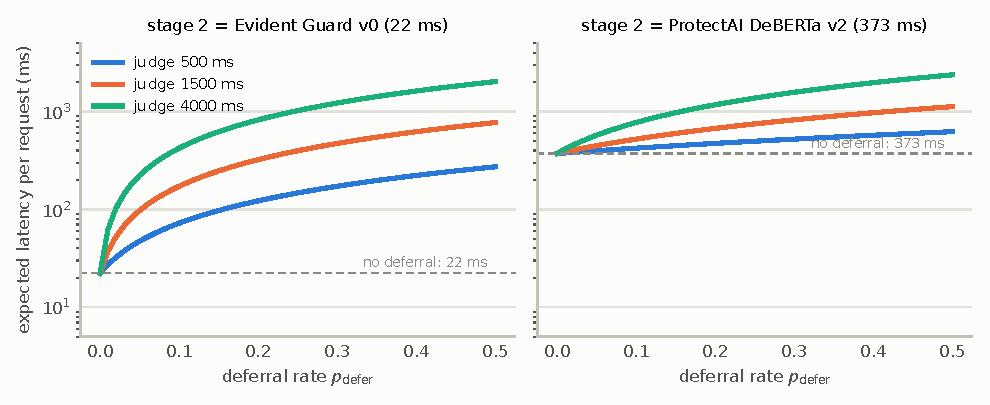
\includegraphics[width=\linewidth]{figures/deferral.pdf}
\caption{Expected latency per request of the cascade as a function of the deferral rate, for the two measured classifiers and three assumed judge latencies (\deferralvariant).}
\label{fig:deferral}
\end{figure}

\begin{algorithm}[t]
\caption{Cascade decision in the shield}
\label{alg:cascade}
\KwIn{input $x$; thresholds; deferral band $[\ell,u)$; block level $b$}
$r_1 \leftarrow \mathrm{Heuristics}(x)$\;
\If{$r_1.\mathrm{level} = \mathrm{critical}$}{\Return block}
$p \leftarrow \mathrm{Classifier}(x)$ (calibrated; on error: $p \leftarrow$ none, or critical if fail-closed)\;
$r_2 \leftarrow \mathrm{LevelOf}(p)$\;
\If{deferral enabled \textbf{and} $\ell \le p < u$ \textbf{and} a judge is configured}{
  $r_3 \leftarrow \mathrm{Judge}(x)$; \quad $r_2 \leftarrow r_3$\;
}
$\mathrm{level} \leftarrow \max(r_1.\mathrm{level}, r_2.\mathrm{level})$\;
\Return block \textbf{if} $\mathrm{level} \ge b$ \textbf{else} allow
\end{algorithm}

\section{Results}
\label{sec:results}

All numbers are from one harness run (\texttt{\resultspath}, \resultsdate) on four CPU cores with no GPU. Four detectors were not measured: Prompt Guard~2 (22M, 86M) is gated behind a licence we had not accepted, Jev needs an API key we did not have, and the LLM judge needs an OpenAI key; their rows are shown as such.

\subsection{Out of distribution}

\Cref{tab:ood} is the main result and \cref{fig:auroc} summarises AUROC across all splits. On sources no model had seen, the regular-expression library at default sensitivity has precision \mregexmediumtestoodprecision{} and a false-positive rate of \mregexmediumtestoodfpr{}, but recall \mregexmediumtestoodrecall{}; raising sensitivity to high buys almost nothing (recall \mregexhightestoodrecall). The $n$-gram logistic regression reaches F$_1$ \mngramlrtestoodfone{} and AUROC \mngramlrtestoodauroc{} at \mngramlrtestoodlatency\ms{} per text. Protect AI's DeBERTa-v3-base reaches F$_1$ \mprotectaidebertavtwotestoodfone{} with AUROC \mprotectaidebertavtwotestoodauroc{} and a false-positive rate of \mprotectaidebertavtwotestoodfpr{}, at \mprotectaidebertavtwotestoodlatency\ms{} per text. \eg{} reaches AUROC \mevidentguardvzerotestoodauroc{}, average precision \mevidentguardvzerotestoodap{}, and at its threshold recall \mevidentguardvzerotestoodrecall{} with a false-positive rate of \mevidentguardvzerotestoodfpr{}; its false-positive rate at 95\% recall is \mevidentguardvzerotestoodfpratrecall{}, against \mprotectaidebertavtwotestoodfpratrecall{} for DeBERTa-base and \mngramlrtestoodfpratrecall{} for the $n$-gram model.

\begin{table}[t]
\centering\scriptsize
\setlength{\tabcolsep}{3.5pt}
\resizebox{\linewidth}{!}{\begin{tabular}{@{}llrrrrrrrrr@{}}
\toprule
Detector & Kind & Thr. & P & R & F$_1$ & FPR & AUROC & AP & FPR@95\%R & ms/text \\
\midrule
regex (low) & rule & 0.01 & 0.991 & 0.584 & 0.735 & 0.010 & 0.790 & 0.849 & 1.000 & 0.08 \\
regex (medium) & rule & 0.01 & 0.990 & 0.604 & 0.750 & 0.011 & 0.799 & 0.856 & 1.000 & 0.09 \\
regex (high) & rule & 0.01 & 0.990 & 0.608 & 0.753 & 0.011 & 0.801 & 0.857 & 1.000 & 0.11 \\
length-only (confound) & confound & 0.50 & 0.553 & 0.508 & 0.530 & 0.722 & 0.336 & 0.538 & 0.987 & 0.00 \\
char n-gram LR & classifier & 0.50 & 0.952 & 0.932 & 0.942 & 0.083 & 0.978 & 0.989 & 0.106 & 0.62 \\
ProtectAI DeBERTa v2 & classifier & 0.50 & 0.996 & 0.983 & 0.990 & 0.006 & 0.998 & 0.998 & 0.002 & 372.54 \\
Evident Guard v0 & classifier & 0.14 & 0.772 & 0.887 & 0.826 & 0.462 & 0.863 & 0.928 & 0.690 & 22.24 \\
\midrule
Prompt Guard 2 (22M) & classifier & \multicolumn{9}{l}{\emph{not measured}: gated model; set HF\_TOKEN after accepting the licence} \\
Prompt Guard 2 (86M) & classifier & \multicolumn{9}{l}{\emph{not measured}: gated model; set HF\_TOKEN after accepting the licence} \\
Jev (TypeSafe) & external & \multicolumn{9}{l}{\emph{not measured}: no TYPESAFE\_API\_KEY configured (user declined to add a key)} \\
LLM judge (gpt-4o-mini) & external & \multicolumn{9}{l}{\emph{not measured}: no OPENAI\_API\_KEY configured} \\
\bottomrule
\end{tabular}
}
\caption{Out-of-distribution split (\ntestood{} rows: \ntestoodattack{} attacks, \ntestoodbenign{} benign; sources \oodsources). Thr.\ is the detector's native threshold; regex scores are an ordinal proxy, so their AUROC and AP rank severities only. Latency is mean ms per text on four CPU cores.}
\label{tab:ood}
\end{table}

\begin{figure}[t]
\centering
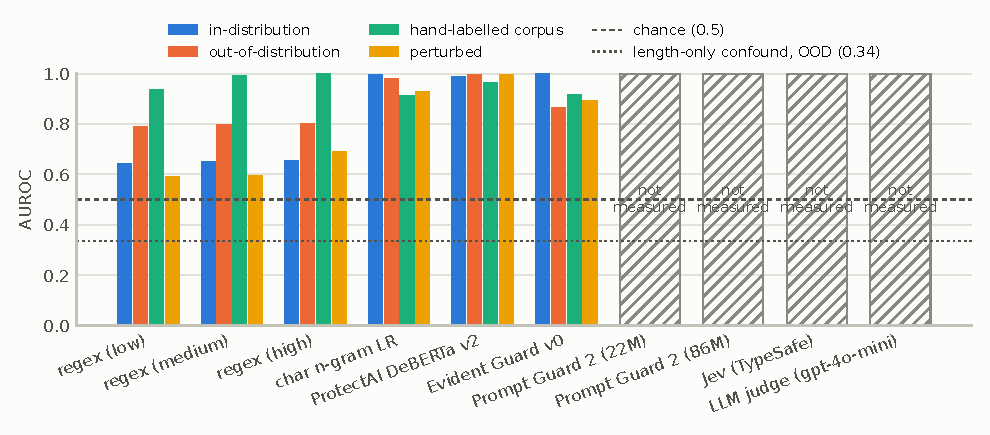
\includegraphics[width=\linewidth]{figures/auroc.pdf}
\caption{AUROC per detector and split. Hatched groups are detectors the run could not measure. The dotted line is the length-only confound on the out-of-distribution split.}
\label{fig:auroc}
\end{figure}

\subsection{In distribution and on the hand-labelled corpus}

\Cref{tab:ind} shows the in-distribution test split. Here \eg{} is the best detector by every ranking metric (AUROC \mevidentguardvzerotestauroc, F$_1$ \mevidentguardvzerotestfone), the $n$-gram model is close behind (AUROC \mngramlrtestauroc), and DeBERTa-base, which was not trained on these sources, has lower recall (\mprotectaidebertavtwotestrecall) at near-perfect precision. The gap between \cref{tab:ind} and \cref{tab:ood} for our model (AUROC \mevidentguardvzerotestauroc{} versus \mevidentguardvzerotestoodauroc) is the central negative result of this paper.

On the hand-labelled corpus (\cref{tab:evident}) the regular-expression library at medium sensitivity reaches F$_1$ \mregexmediumtestevidentfone{}, DeBERTa-base \mprotectaidebertavtwotestevidentfone{}, and \eg{} and the $n$-gram model about \mevidentguardvzerotestevidentfone{}. This ordering is the reverse of the out-of-distribution one and is explained by provenance: the corpus was written while tuning the library, so it is a regression test for the patterns, not an independent benchmark.

\begin{table}[t]
\centering\scriptsize
\setlength{\tabcolsep}{3.5pt}
\resizebox{\linewidth}{!}{\begin{tabular}{@{}llrrrrrrrrr@{}}
\toprule
Detector & Kind & Thr. & P & R & F$_1$ & FPR & AUROC & AP & FPR@95\%R & ms/text \\
\midrule
regex (low) & rule & 0.01 & 0.990 & 0.291 & 0.450 & 0.002 & 0.644 & 0.561 & 1.000 & 0.08 \\
regex (medium) & rule & 0.01 & 0.990 & 0.301 & 0.461 & 0.002 & 0.649 & 0.566 & 1.000 & 0.10 \\
regex (high) & rule & 0.01 & 0.990 & 0.310 & 0.472 & 0.002 & 0.654 & 0.572 & 1.000 & 0.11 \\
length-only (confound) & confound & 0.50 & 0.576 & 0.724 & 0.641 & 0.341 & 0.745 & 0.596 & 0.633 & 0.00 \\
char n-gram LR & classifier & 0.50 & 0.984 & 0.948 & 0.966 & 0.010 & 0.996 & 0.994 & 0.012 & 0.33 \\
ProtectAI DeBERTa v2 & classifier & 0.50 & 0.996 & 0.813 & 0.895 & 0.002 & 0.986 & 0.985 & 0.027 & 294.21 \\
Evident Guard v0 & classifier & 0.14 & 0.976 & 0.985 & 0.980 & 0.016 & 0.999 & 0.999 & 0.002 & 19.59 \\
\bottomrule
\end{tabular}
}
\caption{In-distribution test split (\ntest{} rows). The $n$-gram model and \eg{} were trained on the same sources.}
\label{tab:ind}
\end{table}

\begin{table}[t]
\centering\scriptsize
\setlength{\tabcolsep}{3.5pt}
\resizebox{\linewidth}{!}{\begin{tabular}{@{}llrrrrrrrrr@{}}
\toprule
Detector & Kind & Thr. & P & R & F$_1$ & FPR & AUROC & AP & FPR@95\%R & ms/text \\
\midrule
regex (low) & rule & 0.01 & 1.000 & 0.871 & 0.931 & 0.000 & 0.935 & 0.939 & 1.000 & 0.02 \\
regex (medium) & rule & 0.01 & 0.973 & 0.986 & 0.980 & 0.031 & 0.992 & 0.991 & 0.031 & 0.02 \\
regex (high) & rule & 0.01 & 0.919 & 1.000 & 0.958 & 0.099 & 0.998 & 0.997 & 0.031 & 0.03 \\
length-only (confound) & confound & 0.50 & 0.848 & 0.265 & 0.404 & 0.053 & 0.728 & 0.771 & 0.878 & 0.00 \\
char n-gram LR & classifier & 0.50 & 0.902 & 0.755 & 0.822 & 0.092 & 0.911 & 0.928 & 0.466 & 0.10 \\
ProtectAI DeBERTa v2 & classifier & 0.50 & 0.948 & 0.871 & 0.908 & 0.053 & 0.965 & 0.960 & 0.168 & 15.37 \\
Evident Guard v0 & classifier & 0.14 & 0.859 & 0.789 & 0.823 & 0.145 & 0.915 & 0.933 & 0.435 & 5.82 \\
\bottomrule
\end{tabular}
}
\caption{Hand-labelled corpus (\ntestevident{} rows), the test file the regular-expression library was tuned against.}
\label{tab:evident}
\end{table}

\subsection{Perturbations}

\Cref{tab:perturb} and \cref{fig:perturb} give recall by perturbation type, with the unperturbed recall on both source splits as reference rows. The regular-expression library at default sensitivity keeps about half its recall under a benign prefix (\mpregexmediumbenignprefix) and case flipping (\mpregexmediumcaseflip, since matching is case-insensitive the loss comes from the trigger words being elsewhere in the text), but collapses to around \mpregexmediumtokenbreakspace{} under token breaking, zero-width insertion, homoglyphs and leetspeak, and to \mpregexmediumbasesixfourwrap{} under base64 wrapping.\footnote{The base64 result exposed a pattern bug: the library's encoded-payload pattern required the blob to follow the encoding word immediately, while real framings put ``and follow the instructions inside:'' between them. The fix, with the three harness framings added to the corpus, landed after this run; the regex rows reported here predate it. At high sensitivity a lower-severity pattern already caught \mpregexhighbasesixfourwrap{} of them.} The $n$-gram model degrades gracefully on character-level noise (token break \mpngramlrtokenbreakspace, zero-width \mpngramlrzerowidth) but not on leetspeak (\mpngramlrleetspeak) and not at all on base64 (\mpngramlrbasesixfourwrap), which is expected for a bag of characters. DeBERTa-base is the most robust (worst type: leetspeak at \mpprotectaidebertavtwoleetspeak; base64 at \mpprotectaidebertavtwobasesixfourwrap, presumably because its training data contained such framings). \eg{} holds \mpevidentguardvzeroleetspeak{} on leetspeak and \mpevidentguardvzerotokenbreakspace{} on token breaking, which says the content signal it learned is real even though it does not transfer across sources. The length-only confound scores 1.0 on base64 only because encoding makes the text long.

\begin{table}[t]
\centering\scriptsize
\setlength{\tabcolsep}{3.5pt}
\resizebox{\linewidth}{!}{\begin{tabular}{@{}lrrrrrrr@{}}
\toprule
Perturbation & regex L & regex M & regex H & length & n-gram LR & DeBERTa v2 & EG v0 \\
\midrule
unperturbed, in-distribution & 0.291 & 0.301 & 0.310 & 0.724 & 0.948 & 0.813 & 0.985 \\
unperturbed, OOD & 0.584 & 0.604 & 0.608 & 0.508 & 0.932 & 0.983 & 0.887 \\
\midrule
token break space & 0.107 & 0.120 & 0.128 & 0.295 & 0.873 & 0.917 & 0.895 \\
token break hyphen & 0.110 & 0.120 & 0.128 & 0.655 & 0.833 & 0.932 & 0.902 \\
zero width & 0.087 & 0.098 & 0.105 & 0.655 & 0.882 & 0.932 & 0.915 \\
homoglyph & 0.087 & 0.095 & 0.868 & 0.552 & 0.828 & 0.927 & 0.905 \\
leetspeak & 0.090 & 0.098 & 0.105 & 0.552 & 0.613 & 0.835 & 0.887 \\
case flip & 0.510 & 0.532 & 0.542 & 0.552 & 0.938 & 0.983 & 1.000 \\
benign prefix & 0.512 & 0.535 & 0.542 & 0.682 & 0.830 & 0.927 & 0.940 \\
base64 wrap & 0.000 & 0.000 & 0.665 & 1.000 & 0.018 & 1.000 & 0.762 \\
\bottomrule
\end{tabular}
}
\caption{Recall on perturbed attacks by perturbation type, at each detector's native threshold, with the unperturbed recall on the two source splits for reference. Each type is scored together with the unperturbed benign rows. Columns: regex at low/medium/high sensitivity, the length-only confound, the $n$-gram model, ProtectAI DeBERTa v2 and \eg{} (EG).}
\label{tab:perturb}
\end{table}

\begin{figure}[t]
\centering
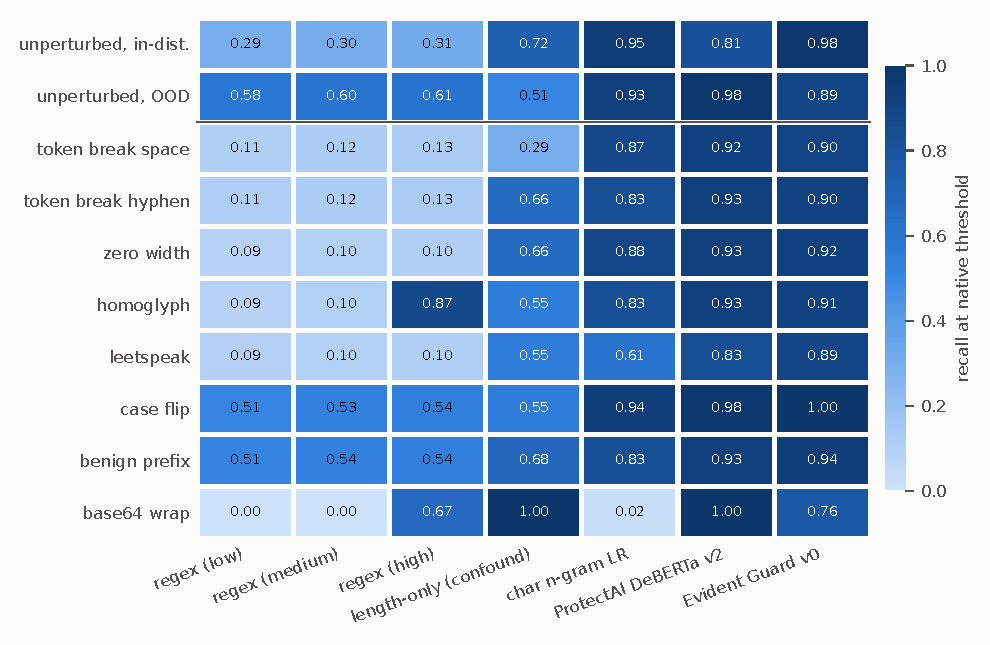
\includegraphics[width=\linewidth]{figures/perturbation.pdf}
\caption{Recall under perturbation (rows) per detector (columns); the two rows above the rule are the unperturbed references.}
\label{fig:perturb}
\end{figure}

\subsection{Length confound}

\Cref{tab:length} reports the protocol of \cref{sec:harness} on the out-of-distribution split (the in-distribution and corpus versions are in the checked-in results). The length-only detector has AUROC \mlengthonlytestauroc{} in distribution, which confirms that length is informative on the training sources, but \mlengthonlytestoodauroc{} out of distribution: on the held-out sources attacks are, if anything, shorter than benign rows, so a length reader is worse than chance. On the length-matched subset every detector's AUROC holds or rises: the $n$-gram model from \mngramlrtestoodauroc{} to \mngramlrtestoodlmauroc{}, DeBERTa-base from \mprotectaidebertavtwotestoodauroc{} to \mprotectaidebertavtwotestoodlmauroc{}, \eg{} from \mevidentguardvzerotestoodauroc{} to \mevidentguardvzerotestoodlmauroc{}, and the regular-expression library from \mregexmediumtestoodauroc{} to \mregexmediumtestoodlmauroc. Nothing in \cref{tab:ood} is a length shortcut.

\begin{table}[t]
\centering\scriptsize
\setlength{\tabcolsep}{4pt}
\resizebox{\linewidth}{!}{\begin{tabular}{@{}lrrrrrl@{}}
\toprule
Detector & AUROC & F$_1$ & AUROC$_\mathrm{m}$ & F$_{1,\mathrm{m}}$ & $n_\mathrm{m}$ & AUROC by length quartile \\
\midrule
regex (low) & 0.790 & 0.735 & 0.860 & 0.836 & 886 & 0.70 / 0.83 / 0.89 / 0.83 \\
regex (medium) & 0.799 & 0.750 & 0.865 & 0.844 & 886 & 0.71 / 0.84 / 0.89 / 0.84 \\
regex (high) & 0.801 & 0.753 & 0.869 & 0.848 & 886 & 0.71 / 0.84 / 0.90 / 0.85 \\
length-only (confound) & 0.336 & 0.530 & 0.577 & 0.623 & 886 & 0.68 / 0.68 / 0.53 / 0.61 \\
char n-gram LR & 0.978 & 0.942 & 0.993 & 0.954 & 886 & 0.98 / 0.99 / 0.99 / 0.99 \\
ProtectAI DeBERTa v2 & 0.998 & 0.990 & 0.997 & 0.976 & 886 & 1.00 / 1.00 / 1.00 / 0.98 \\
Evident Guard v0 & 0.863 & 0.826 & 0.928 & 0.791 & 886 & 0.84 / 0.90 / 0.93 / 0.98 \\
\bottomrule
\end{tabular}
}
\caption{Length-confound check on the out-of-distribution split. Subscript m: length-matched subset ($n_\mathrm{m}$ rows). Quartiles are of character length within the split, short to long.}
\label{tab:length}
\end{table}

\subsection{Latency}

\Cref{fig:latency} plots mean latency against out-of-distribution AUROC. The regular-expression library costs about a tenth of a millisecond, the $n$-gram model under a millisecond, \eg{} about \mevidentguardvzerotestoodlatency\ms{} and DeBERTa-base about \mprotectaidebertavtwotestoodlatency\ms{} per text in the Python harness; in the Node.js shield the two neural models measured 12 to 14\ms{} and 23\ms{} respectively after a one-time load of 1.8\,s and 17\,s. The 95th-percentile latencies are in the tables.

\begin{figure}[t]
\centering
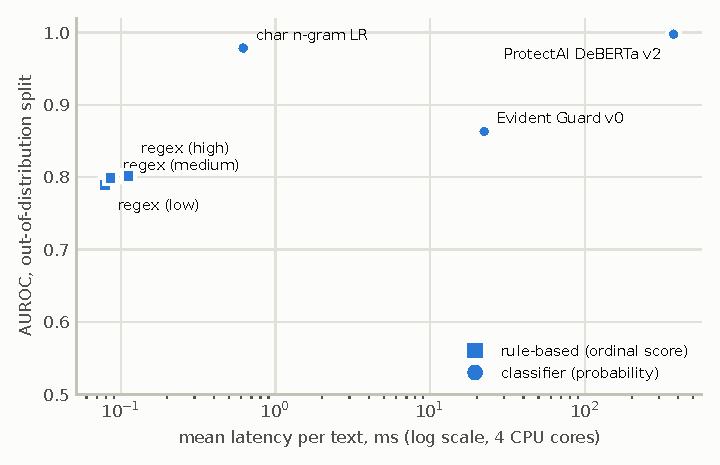
\includegraphics[width=0.72\linewidth]{figures/latency_auroc.pdf}
\caption{Mean latency per text (log scale) against out-of-distribution AUROC. The length-only confound is omitted (its latency is zero and its AUROC below chance).}
\label{fig:latency}
\end{figure}

\section{Discussion}
\label{sec:discussion}

\paragraph{Heuristics are a filter, not a defence.} The regular-expression library's out-of-distribution precision of \mregexmediumtestoodprecision{} means that when it fires it is almost always right, and its \mregexmediumtestoodlatency\ms{} cost means it can run on every request. Its recall of \mregexmediumtestoodrecall{} means that on its own it misses two attacks in five on unseen data, and its collapse under token-level perturbation means an adversary who knows it exists evades it trivially. Both facts argue for the same architecture: use it as Stage~1 to resolve clear cases at no cost and to stop early on critical matches, and never as the only stage. We note that the perturbations that defeat it (homoglyphs, zero-width characters, token breaks) are ones a normalisation pass could partly undo before matching; we have not added one, and it would not help against base64 or paraphrase.

\paragraph{Why our model overfits, and what to do about it.} \eg{} was trained on two attack sources and two benign sources and evaluated on two others. Its in-distribution AUROC of \mevidentguardvzerotestauroc{} and out-of-distribution AUROC of \mevidentguardvzerotestoodauroc{} bracket the $n$-gram model's \mngramlrtestauroc{} and \mngramlrtestoodauroc{}: the neural model learned the training sources better and the test sources worse. Two decisions compounded this. First, the threshold was chosen to maximise F$_1$ on an in-distribution validation set, landing at 0.14; a threshold that low, applied to a shifted score distribution, produced an out-of-distribution false-positive rate of \mevidentguardvzerotestoodfprpct\%. Choosing the threshold at a target false-positive rate, which is what an operator actually specifies, would have been the right criterion. Second, three epochs on \ntrain{} rows with no source-level validation let the model fit source-specific style. The fixes are cheap and we list them as next steps: hold out a different source for validation, train on all but one source in rotation, and select the threshold by target false-positive rate. The perturbation rows suggest the content signal is worth keeping: the model is robust to leetspeak and token breaking in a way the $n$-gram model is not.

\paragraph{The bar.} Protect AI's DeBERTa-v3-base is the best detector in every out-of-distribution column and the most robust to perturbation, at a cost of \mprotectaidebertavtwotestoodlatency\ms{} per text on CPU, roughly seventeen times our model. For a gateway serving interactive traffic that is a real cost; for a release gate run in CI it is irrelevant. The honest summary is that, on this benchmark and today, a team should run DeBERTa-base as Stage~2 unless latency forbids it, and our model's contribution is the calibration-and-export path that lets any such classifier, including that one, run inside the Node.js shield with a temperature applied.

\paragraph{The $n$-gram surprise.} A character $n$-gram logistic regression that trains in seconds and scores in half a millisecond reaches out-of-distribution F$_1$ \mngramlrtestoodfone{}. It is also, on the length-matched subset, essentially as good as DeBERTa-base by AUROC (\mngramlrtestoodlmauroc{} versus \mprotectaidebertavtwotestoodlmauroc). Its weaknesses are precise and expected: leetspeak and base64, which destroy its character statistics. Anyone building a classifier for this task should train this baseline first; we did not, and would have calibrated our expectations better if we had.

\paragraph{What the length check rules out.} Public injection datasets differ from benign instruction data in length, and a classifier that exploited that would look good in distribution and fail in production. The length-only baseline being below chance out of distribution, and every detector keeping its AUROC under length matching, rule that explanation out for all four measured detectors. This check cost one logistic regression and we recommend it for any detector evaluation on mixed public sources.

\paragraph{Calibration, deferral and confident errors.} Biswas~\cite{biswas2026confidently} reports that public detectors miss attacks with confidence near one under shift. Temperature scaling cannot fix that: it rescales all logits by one constant and cannot move a confident miss into the deferral band. What the band does buy is a principled budget for the cases the classifier itself flags as uncertain, and a place to attach a judge without paying for it on every request. The empirical shape of that trade-off, accuracy as a function of deferral rate on real scores, is the measurement we most want and did not make, because the harness stores aggregates; adding per-row scores is a small change.

\section{Limitations}
\label{sec:limitations}

\begin{itemize}
\item \textbf{Single seed, single run.} Every number is from one training run and one harness run; we report no variance.
\item \textbf{Small data and CPU training.} \ntrain{} training rows, maximum sequence length 128, 33 minutes of CPU. Attacks longer than 128 tokens are truncated at training time.
\item \textbf{Synthetic perturbations and no adaptive adversary.} The eight perturbations approximate TokenBreak-style attacks with fixed rules on a fixed trigger list; a real attacker optimises against the deployed detector.
\item \textbf{Three detectors not measured.} Prompt Guard~2 (gated), Jev (API key) and an LLM judge (API key) have adapters but no numbers here; the comparison with the strongest commercial and open baselines is therefore incomplete, and the published Jev figures we quote are the preprint's, not ours.
\item \textbf{The corpus favours the regular-expression library.} \texttt{test\_evident} was written while tuning the patterns and should be read as a regression test.
\item \textbf{The base64 fix postdates the run.} The regular-expression rows in the perturbation table were measured before the encoded-payload pattern was corrected.
\item \textbf{Threshold selection.} \eg's threshold was selected by in-distribution F$_1$, which we argue above is the wrong criterion; the reported out-of-distribution false-positive rate is partly a consequence of that choice rather than of the model's ranking quality, which AUROC and the length-matched AUROC (\mevidentguardvzerotestoodlmauroc) capture better.
\item \textbf{Regex AUROC is indicative.} The ordinal proxy score makes AUROC and average precision for the regular-expression detectors a ranking of severities, not of probabilities.
\item \textbf{Scope.} The release-gate formulation covers direct injection through a test input and leaks through canaries; it does not model multi-turn attacks or tool-mediated indirect injection beyond what a test author writes into $x$.
\end{itemize}

\paragraph{Ethics and dual use.} The harness and corpus contain attack strings. All are drawn from public datasets or are short, generic phrasings already in wide circulation, and the perturbation code implements well-known obfuscations rather than novel attacks. They are used to measure and improve defences; nothing here lowers the cost of an attack beyond what a search for the cited datasets would. Model outputs are never stored by the release gate unless the user opts in.

\section{Reproducibility}
\label{sec:repro}

Everything runs on CPU. The commands below reproduce the data, the model and every table and figure in this paper from the public repository.

\begin{verbatim}
pnpm install --frozen-lockfile   # Node workspace: detectors, cli, shield, gateway
cd packages/evals
python3 -m venv .venv && . .venv/bin/activate
pip install torch --index-url https://download.pytorch.org/whl/cpu
pip install -r requirements.txt
python -m evals.data      # download, dedupe, split -> data/*.jsonl, manifest.json
python -m evals.perturb   # perturb test attacks     -> data/test_perturbed.jsonl
python -m evals.train     # fine-tune, calibrate, export -> models/evident-guard-v0/
python -m evals.run       # score every detector     -> results/<date>/metrics.json
cd ../../paper && make final     # figures, tables, this PDF
\end{verbatim}

\noindent The model directory contains \texttt{model.onnx} (and a hard link at \texttt{onnx/model.onnx} for Transformers.js), the tokenizer files, \texttt{config.json} with \texttt{id2label} $\{0\colon \text{BENIGN}, 1\colon \text{INJECTION}\}$, and \texttt{calibration.json}:
\begin{verbatim}
{"model": "evident-guard-v0",
 "base_model": "microsoft/deberta-v3-xsmall",
 "temperature": 1.6337, "threshold": 0.14, "max_length": 128,
 "positive_label": "INJECTION", "val_macro_f1": 0.9836,
 "ece_before": 0.0125, "ece_after": 0.0072}
\end{verbatim}
Consumers compute $\mathrm{softmax}(z/T)[1]$ and compare with the threshold. To use the model in the shield:
\begin{verbatim}
new Shield({
  analyzers: ['heuristic', 'ml'],
  ml: { backend: 'transformers', model: '/path/to/evident-guard-v0',
        localFilesOnly: true, threshold: 0.5 },
  deferral: { enabled: true, lower: 0.3, upper: 0.7 },
  llm: { provider: 'openai' },
})
\end{verbatim}
Setting \texttt{HF\_TOKEN}, \texttt{TYPESAFE\_API\_KEY} or \texttt{OPENAI\_API\_KEY} before \texttt{python -m evals.run} fills in the rows that are not measured here. The harness's unit tests (\texttt{pytest}) and the corpus test of the pattern library (\texttt{pnpm test}) run without network access.

\printbibliography

\end{document}
